\documentclass[aspectratio=169]{beamer}


\usepackage{booktabs}
\usepackage{graphicx}
\usepackage{amsmath}
\usepackage{tikz}
\usetikzlibrary{positioning,arrows.meta}
\usepackage{xcolor}
\usepackage[T1]{fontenc}
\usepackage{helvet}
\renewcommand{\familydefault}{\sfdefault}
\usefonttheme{professionalfonts}
\graphicspath{{figures/}}

\setbeamertemplate{navigation symbols}{}
\setbeamertemplate{blocks}[rounded][shadow=false]

% ---- semantic paradigm colours (Okabe-Ito, colour-blind safe) ----
\definecolor{coltemporal}{HTML}{E69F00}   % temporal methods
\definecolor{colspatial}{HTML}{009E73}    % spatial methods
\definecolor{colgraph}{HTML}{0072B2}      % spatiotemporal graph (highlight)
\definecolor{colmask}{HTML}{0072B2}

\setbeamercolor{structure}{fg=colgraph}
\setbeamercolor{title}{fg=colgraph}
\setbeamercolor{frametitle}{fg=colgraph,bg=white}
\setbeamercolor{itemize item}{fg=colgraph}
\setbeamercolor{itemize subitem}{fg=colgraph}
\setbeamerfont{frametitle}{size=\large,series=\bfseries}
\setbeamertemplate{frametitle}{%
  \vspace*{1.1ex}\insertframetitle\par
  \vspace*{0.3ex}{\color{colgraph}\rule{\textwidth}{1pt}}\vspace*{0.4ex}}

\setbeamercolor{footcol}{fg=black!55}
\setbeamertemplate{footline}{%
  \leavevmode\hbox to\paperwidth{\usebeamercolor[fg]{footcol}%
  \hspace{1.5em}\footnotesize\insertshorttitle\hfill
  \footnotesize\insertframenumber\,/\,\inserttotalframenumber\hspace{1.5em}}%
  \vspace{1.2ex}}

\AtBeginSection[]{%
  \begin{frame}[plain]
    \centering\vfill
    {\color{colgraph}\Large\bfseries\insertsectionhead}\\[1.2ex]
    {\color{black!40}\rule{0.4\textwidth}{1pt}}
    \vfill
  \end{frame}}

\newcommand{\plegend}{{\footnotesize%
  \textcolor{coltemporal}{$\blacksquare$}~temporal\quad
  \textcolor{colspatial}{$\blacksquare$}~spatial\quad
  \textcolor{colgraph}{$\blacksquare$}~spatiotemporal graph}}
\newcommand{\take}[1]{\vspace{0.6ex}\begin{center}\textbf{\color{colgraph}#1}\end{center}}
\newcommand{\maskgrid}[1]{%
 \begin{tikzpicture}[scale=0.30]
  \foreach \x in {0,1,2,3,4,5} \foreach \y in {0,1,2,3,4,5} \draw[gray!45] (\x,\y) rectangle ++(1,1);
  \foreach \x/\y in {#1} \fill[colmask!75] (\x,\y) rectangle ++(1,1);
 \end{tikzpicture}}

\title[Spatiotemporal Graph Wave Modelling]{A Spatiotemporal Graph Approach to Buoy Wave-Field Imputation, Forecasting, and Wave Energy}

\begin{document}

% ===================== TITLE =====================
\begin{frame}[plain]
  \vfill
  \begin{center}
    {\color{colgraph}\Large\bfseries A Spatiotemporal Graph Approach to Buoy\\[0.3ex]
     Wave-Field Imputation, Forecasting, and Wave Energy}\\[2.0ex]
    {\large Richel Attafuah}\\[0.4ex]
    {\small Department of Statistics, Miami University}\\[1.6ex]
    {\footnotesize Advisor: Prof.\ Mahsa Ashouri}\\[0.3ex]
    {\footnotesize Co-authors: Prof.\ Miao Wang \quad Shirin Besati (UNC Charlotte)}\\[1.6ex]
    {\footnotesize \today \quad$\cdot$\quad Target venue: \emph{Renewable Energy}}
  \end{center}
  \vfill
\end{frame}

% ===================== THESIS =====================
\begin{frame}
  \vfill
  \begin{center}\large
  Buoy networks go dark. Neither purely \textcolor{coltemporal}{temporal} nor purely
  \textcolor{colspatial}{spatial} methods can recover them.\\[1.5ex]
  A \textcolor{colgraph}{\bfseries spatiotemporal graph} model recovers both scattered gaps
  \emph{and} blacked-out stations, forecasts 12--24\,h ahead at about
  \textcolor{colgraph}{\bfseries 3$\times$} classical skill, and feeds a wave-power derivation.
  \end{center}
  \vfill
  \note{This is the whole talk in one sentence. Everything after is evidence for each clause: recovers both regimes (imputation), 3x skill (forecasting), wave power (energy). Say it slowly.}
\end{frame}

% ===================== OUTLINE =====================
\begin{frame}{Outline}
  \begin{enumerate}
    \item[\textbf{I}] Problem \& Data
    \item[\textbf{II}] Evaluation Design
    \item[\textbf{III}] Imputation
    \item[\textbf{IV}] Forecasting
    \item[\textbf{V}] Wave Energy
  \end{enumerate}
  \vfill\plegend
  \note{Five parts. The hinge is Part III slide "the dichotomy" -- flag that this is where the argument turns. Colour code is fixed for the whole deck: orange temporal, green spatial, blue graph.}
\end{frame}

% ##################### PART I #####################
\section{Part I \textperiodcentered\ Problem \& Data}

\begin{frame}{Motivation: resource assessment needs continuous records}
  \begin{itemize}
    \item Wave-energy siting integrates power over \emph{years} of hourly sea state.
    \item NDBC records are \emph{not} continuous. Two distinct failure modes:
    \begin{itemize}
      \item[--] \textbf{Scattered dropouts} --- isolated missing hours.
      \item[--] \textbf{Whole-station outages} --- a buoy goes dark for weeks.
    \end{itemize}
    \item These are different problems and demand different recovery skills.
  \end{itemize}
  \note{Frame the applied stakes first: you cannot integrate power over gaps. The two failure modes preview the two evaluation regimes. The whole-station outage is the one the committee asked us to centre.}
\end{frame}

\begin{frame}{Station selection: a documented cascade}
  \begin{center}
  \begin{tabular}{r l}
    \toprule
    Stage & Count \\
    \midrule
    Wave-plausible stations (crawl) & \textbf{[VERIFY]} \\
    Audited with computed coverage & \textbf{872} \\
    Have any WVHT observations & \textbf{283} \\
    Retained: $\ge$70\% WVHT coverage, $\ge$3 years & \textbf{140} \\
    \bottomrule
  \end{tabular}
  \end{center}
  \take{The filter is a fixed rule, not a hand-pick: $\ge$70\% coverage over $\ge$3 years $\rightarrow$ 140 stations.}
  \note{The rule is pre-committed and reproducible from coverage\_thresholds.csv (the 0.70 row gives 140 at every min-years cut). The 1,176 pre-audit figure is not in a committed file -- flagged VERIFY; the auditable chain is 872 to 283 to 140.}
\end{frame}

\begin{frame}{The retained network spans every U.S. basin}
  \begin{center}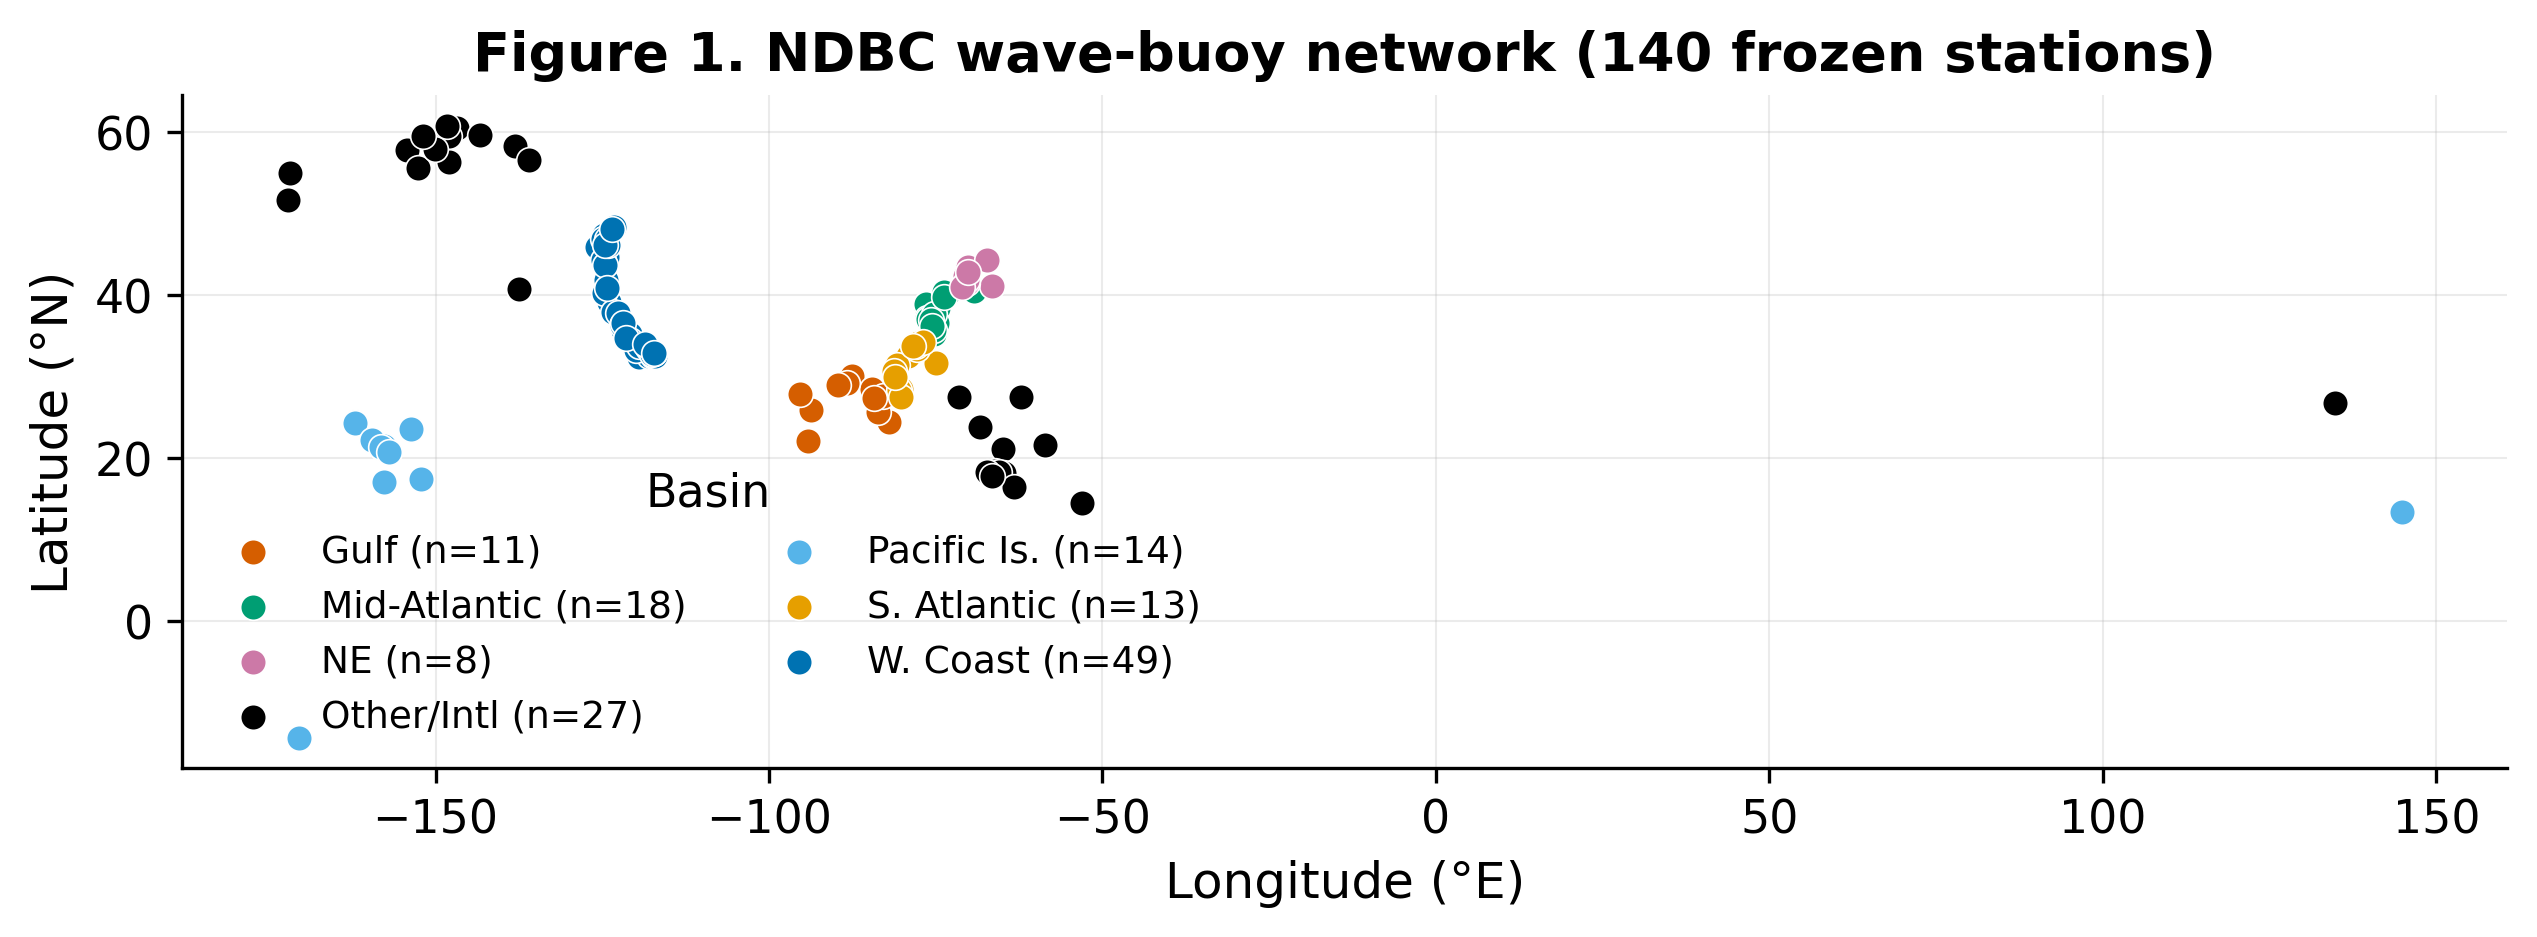
\includegraphics[width=\textwidth,height=0.64\textheight,keepaspectratio]{fig1_station_map.png}\end{center}
  \take{National coverage across multiple ocean basins --- the spatial spread the graph will exploit.}
  \note{Point out the basin clusters: West Coast, Pacific Islands, Gulf, the Atlantic seaboard. The graph edges will live inside these clusters.}
\end{frame}

\begin{frame}{The data as one tensor}
  \begin{center}\large
  $[\,43{,}824\ \text{hours}\;\times\;140\ \text{stations}\;\times\;3\ \text{features}\,]$\\[1ex]
  \normalsize hourly, 2021--2025
  \end{center}
  \begin{itemize}
    \item Targets: \textbf{WVHT} (significant wave height), \textbf{APD} (average period).
    \item Predictor feature: \textbf{DPD} (dominant period) --- \emph{not} a target.
  \end{itemize}
  \take{Committee redirect: DPD was demoted from target to feature; we model WVHT and APD.}
  \note{The DPD demotion came from an earlier committee meeting -- surface it proactively; it shows we act on feedback. Three features in the tensor, two are scored.}
\end{frame}

\begin{frame}{Missingness is structured, not random}
  \begin{center}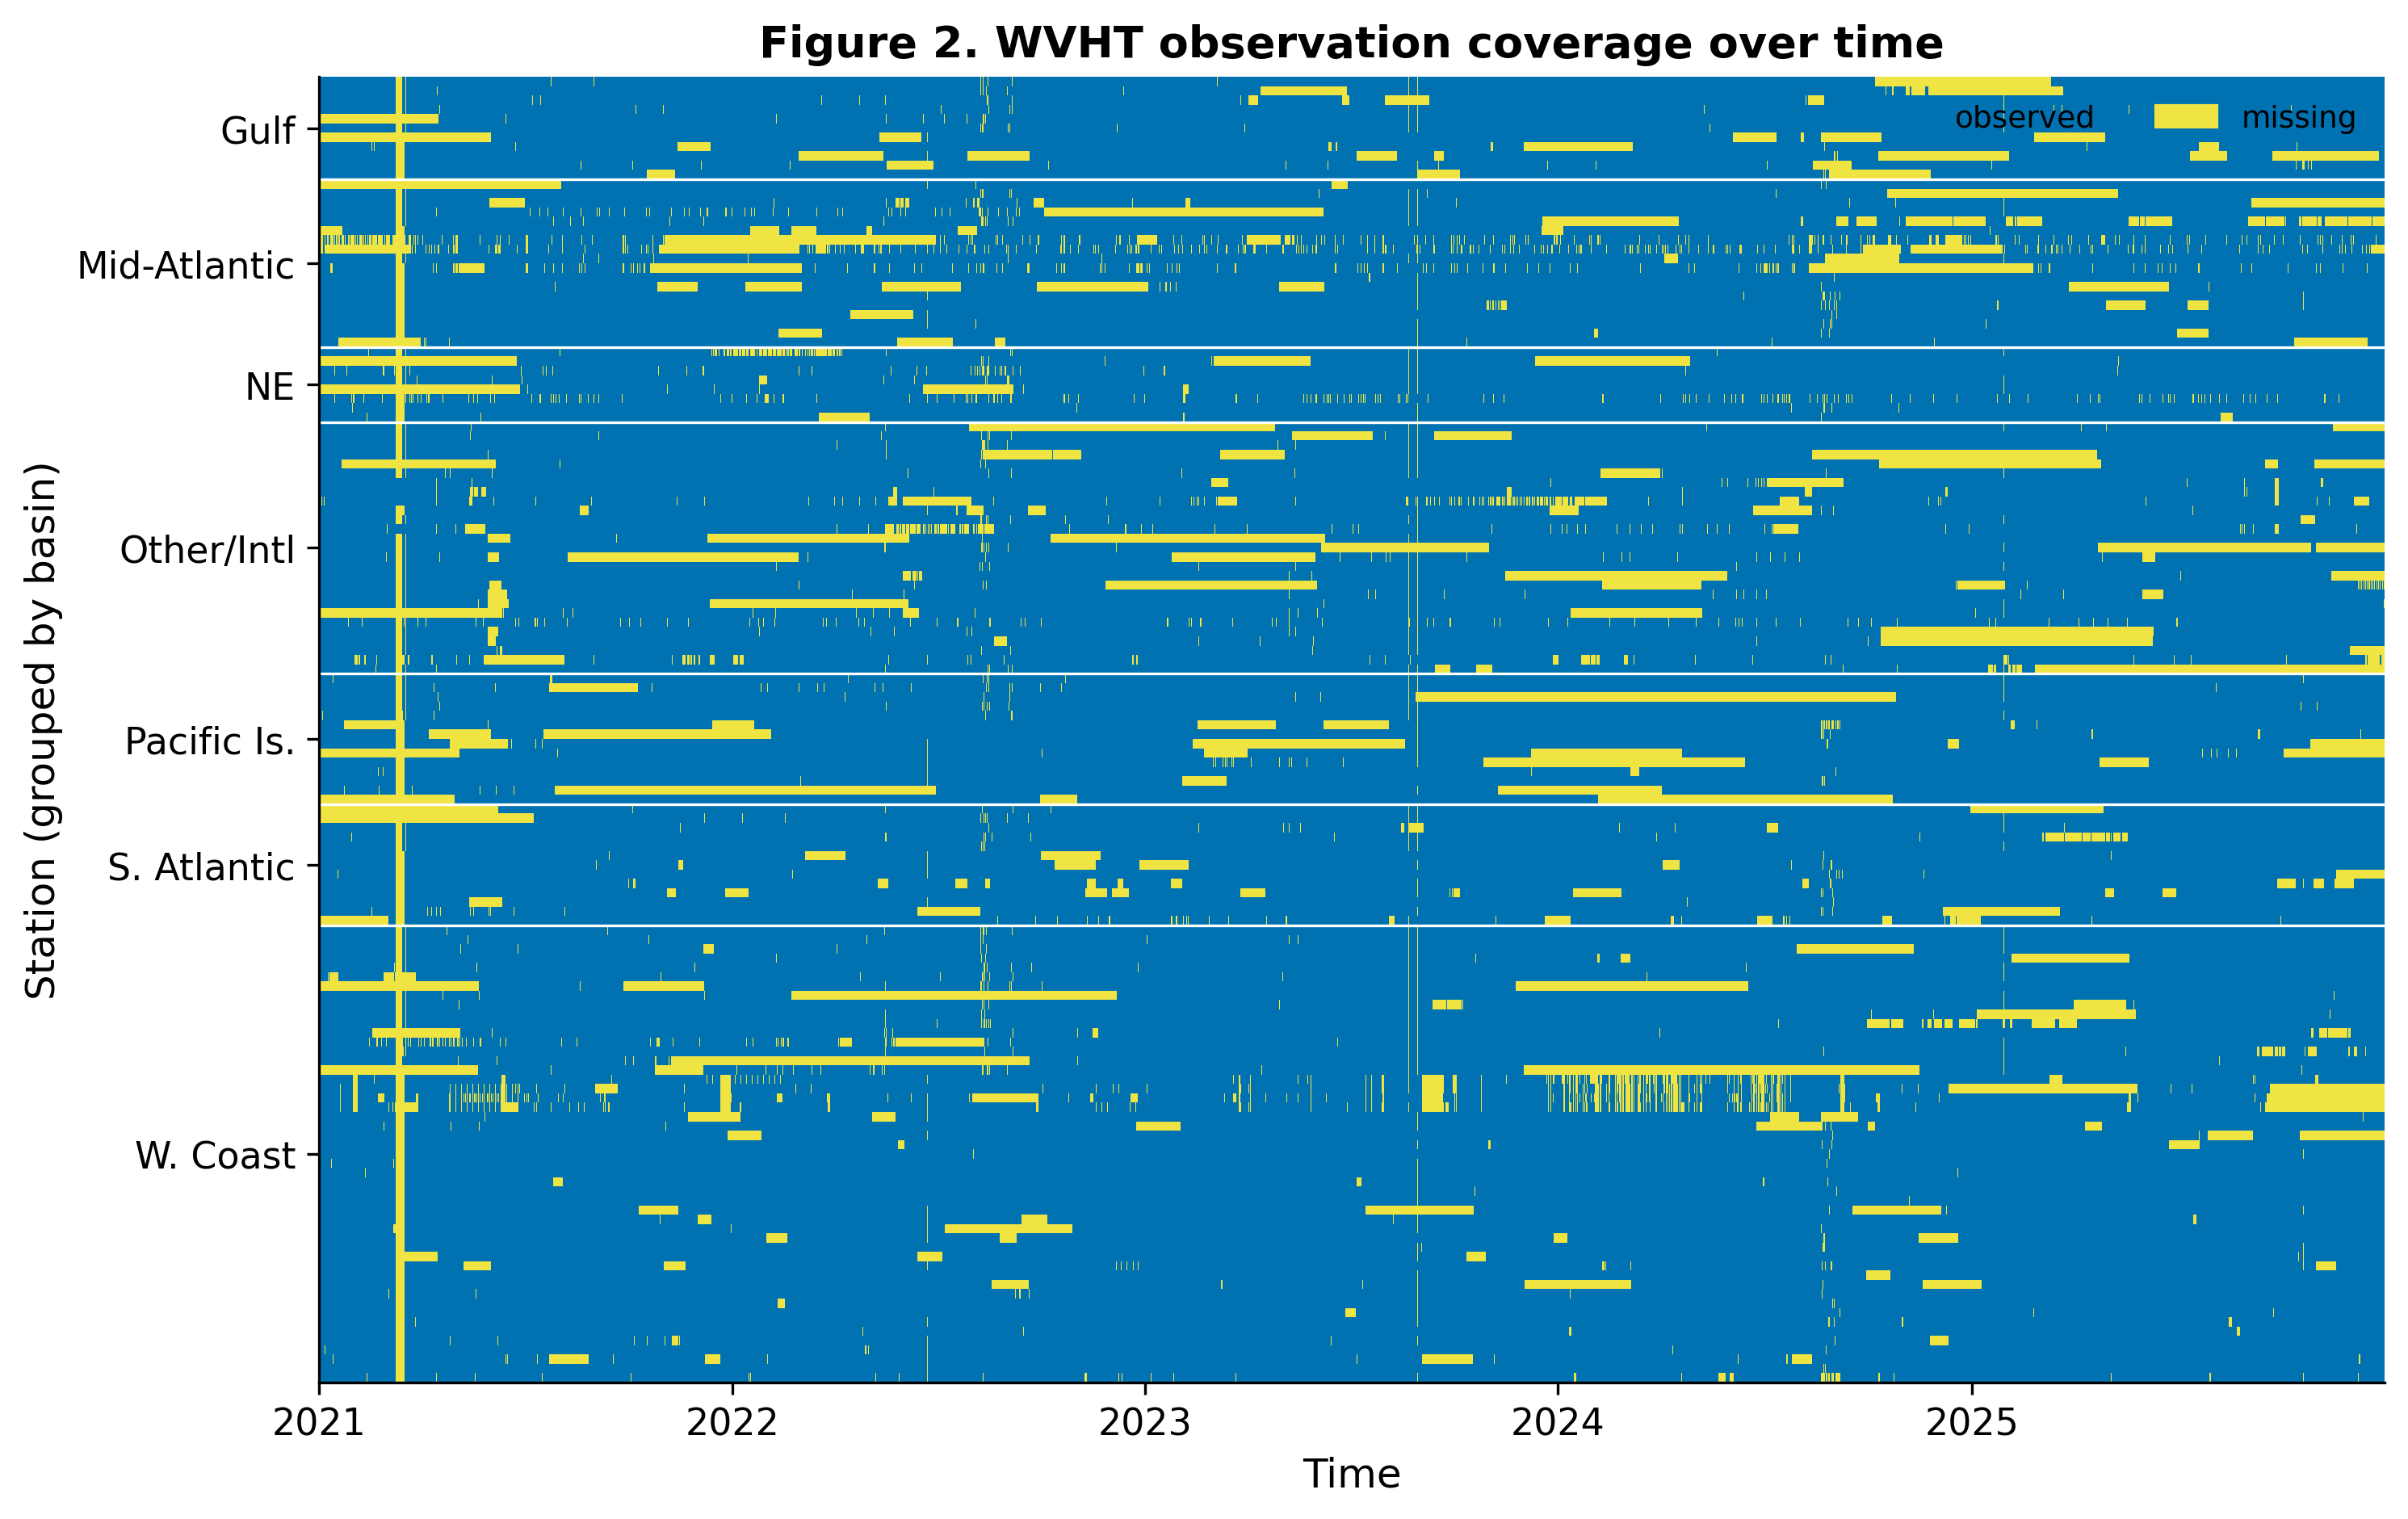
\includegraphics[width=\textwidth,height=0.60\textheight,keepaspectratio]{fig2_missingness.png}\end{center}
  \take{The white bands are whole stations going dark --- that is the centerpiece scenario.}
  \note{Do not let them read this as random noise. The vertical/horizontal white bands are outages. This heatmap is the visual justification for a dedicated station-outage regime.}
\end{frame}

\begin{frame}{Preprocessing: three decisions, each justified}
  \begin{itemize}
    \item \textbf{log1p on WVHT only} --- right-skewed (skew $\approx$~\textbf{[VERIFY]}); periods are near-symmetric, kept in natural units.
    \item \textbf{DPD, APD in natural units} --- no transform needed.
    \item \textbf{Wind excluded} --- \textbf{[VERIFY]} of 140 stations have no anemometer: structurally missing-not-at-random, so wind is dropped rather than imputed.
  \end{itemize}
  \note{Each choice pre-empts a statistician's question. The skew value and the anemometer count are not in a committed CSV -- both flagged VERIFY; fill from the EDA log before the defence. The wind point is a MNAR argument, say it in those words.}
\end{frame}

% ##################### PART II #####################
\section{Part II \textperiodcentered\ Evaluation Design}

\begin{frame}{The protocol was written before any model existed}
  \begin{itemize}
    \item \texttt{EVALUATION.md} is pre-registered and version-controlled.
    \item It binds every experiment: no result counts unless it conforms.
    \item \textbf{Temporal split:} train 2021--2023 \;$\cdot$\; validate 2024 \;$\cdot$\; test 2025.
  \end{itemize}
  \take{Pre-registration removes the ``you tuned to the test set'' objection.}
  \note{Emphasise the ordering: the protocol predates the models, and it is a committed file with git history to prove it. The temporal split never pools timestamps.}
\end{frame}

\begin{frame}{Imputation evaluation: hide-and-recover}
  \begin{center}
  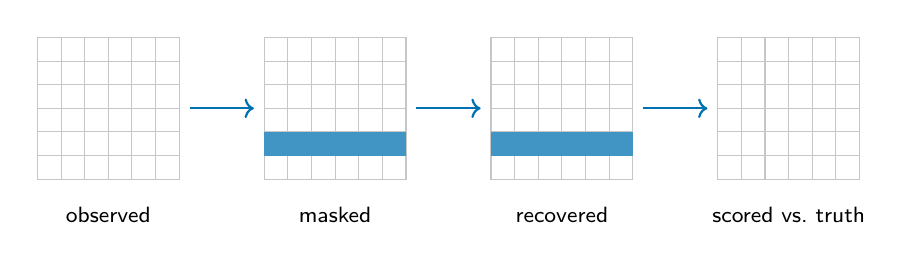
\begin{tikzpicture}[scale=0.9, every node/.style={font=\footnotesize}]
    \node (a) at (0,0) {\maskgrid{}};
    \node[below=0.1cm of a] {observed};
    \node (b) at (3.2,0) {\maskgrid{0/1,1/1,2/1,3/1,4/1,5/1}};
    \node[below=0.1cm of b] {masked};
    \node (c) at (6.4,0) {\maskgrid{0/1,1/1,2/1,3/1,4/1,5/1}};
    \node[below=0.1cm of c] {recovered};
    \node (d) at (9.6,0) {\maskgrid{}};
    \node[below=0.1cm of d] {scored vs.\ truth};
    \foreach \s/\t in {a/b,b/c,c/d} \draw[->,thick,colgraph] (\s.east) -- (\t.west);
  \end{tikzpicture}
  \end{center}
  \begin{itemize}
    \item Hide \emph{observed} cells, recover, score in physical units against held-out truth.
    \item \textbf{Every method passes through identical fixed masks.}
  \end{itemize}
  \note{The fixed-mask point is the fairness guarantee: paradigms are compared on exactly the same held-out cells. Scores are MAE in metres / seconds, not normalised.}
\end{frame}

\begin{frame}{Three missingness mechanisms}
  \begin{columns}[T]
    \column{0.33\textwidth}\centering \maskgrid{0/3,2/5,4/1,1/0,5/4,3/3,2/2}\\[0.5ex]\textbf{MCAR}\\{\footnotesize scattered}
    \column{0.33\textwidth}\centering \maskgrid{2/4,3/4,4/4}\\[0.5ex]\textbf{Block}\\{\footnotesize contiguous}
    \column{0.33\textwidth}\centering \maskgrid{0/1,1/1,2/1,3/1,4/1,5/1}\\[0.5ex]\textbf{Station-outage}\\{\footnotesize whole buoy dark}
  \end{columns}
  \take{Station-outage --- a whole buoy dark --- is the centerpiece, per committee direction.}
  \note{Rows are stations, columns are time. MCAR sprinkles, block removes a run in one station, outage removes an entire station. Rates 10/30/50\% for the first two.}
\end{frame}

\begin{frame}{Why hide values we already have?}
  \begin{enumerate}
    \item You cannot compute error against a value that does not exist.
    \item Field standard: Cini et al.\ (ICLR 2022), Cao et al.\ (NeurIPS 2018), Tashiro et al.\ (NeurIPS 2021), Du et al.\ (2023), Wang et al.\ (2024).
    \item The trained model \emph{does} impute the real gaps --- this measures how far to trust those imputations.
    \item The outage mask reproduces the \emph{actual} observed failure mode.
  \end{enumerate}
  \note{This is a question magnet -- give it a whole slide. Point (1) is the logical necessity, (2) is precedent, (3) is the practical payoff, (4) is realism. Have the five citations ready.}
\end{frame}

% ##################### PART III #####################
\section{Part III \textperiodcentered\ Imputation}

\begin{frame}{Why a graph? Nearby buoys inform each other}
  \begin{center}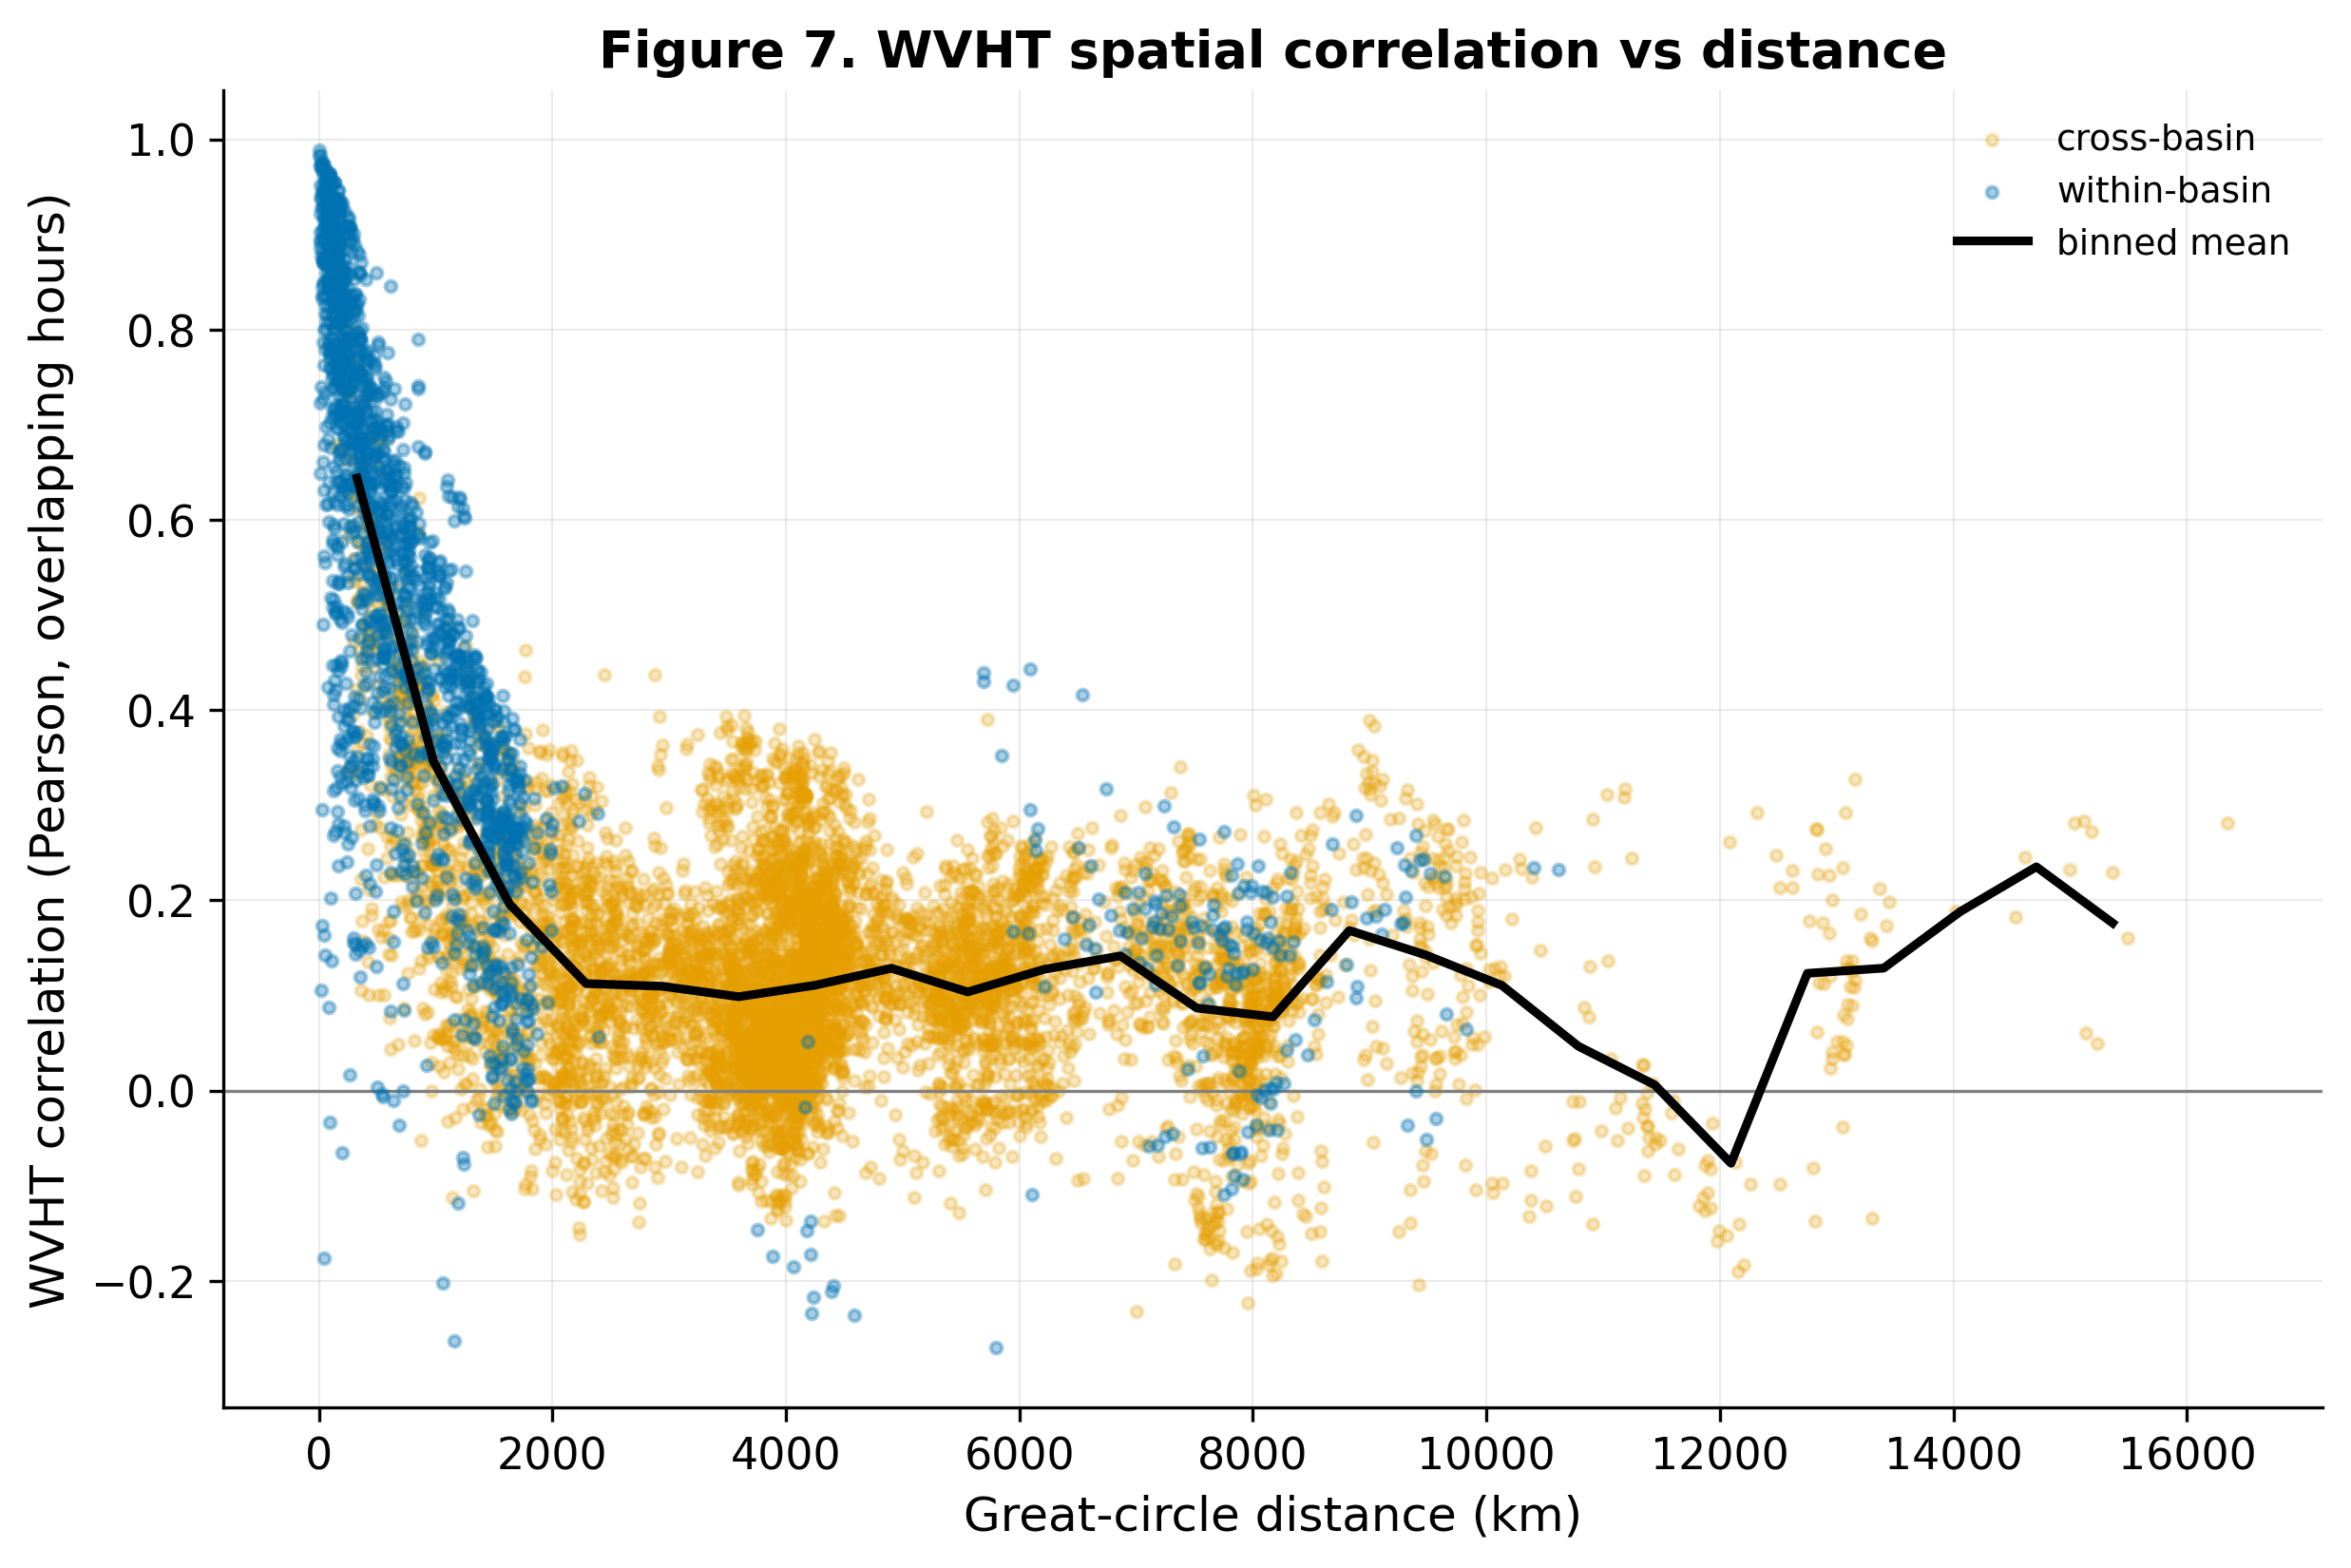
\includegraphics[width=\textwidth,height=0.60\textheight,keepaspectratio]{fig7_corr_distance.png}\end{center}
  \take{Correlation decays with distance --- the load-bearing empirical case for a graph.}
  \note{This is the single most important justification slide. If neighbours were uninformative the graph would be pointless; this figure shows they are strongly correlated at short range, within basin especially.}
\end{frame}

\begin{frame}{Graph construction, with data-quality diligence}
  \begin{columns}[T]
    \column{0.54\textwidth}
    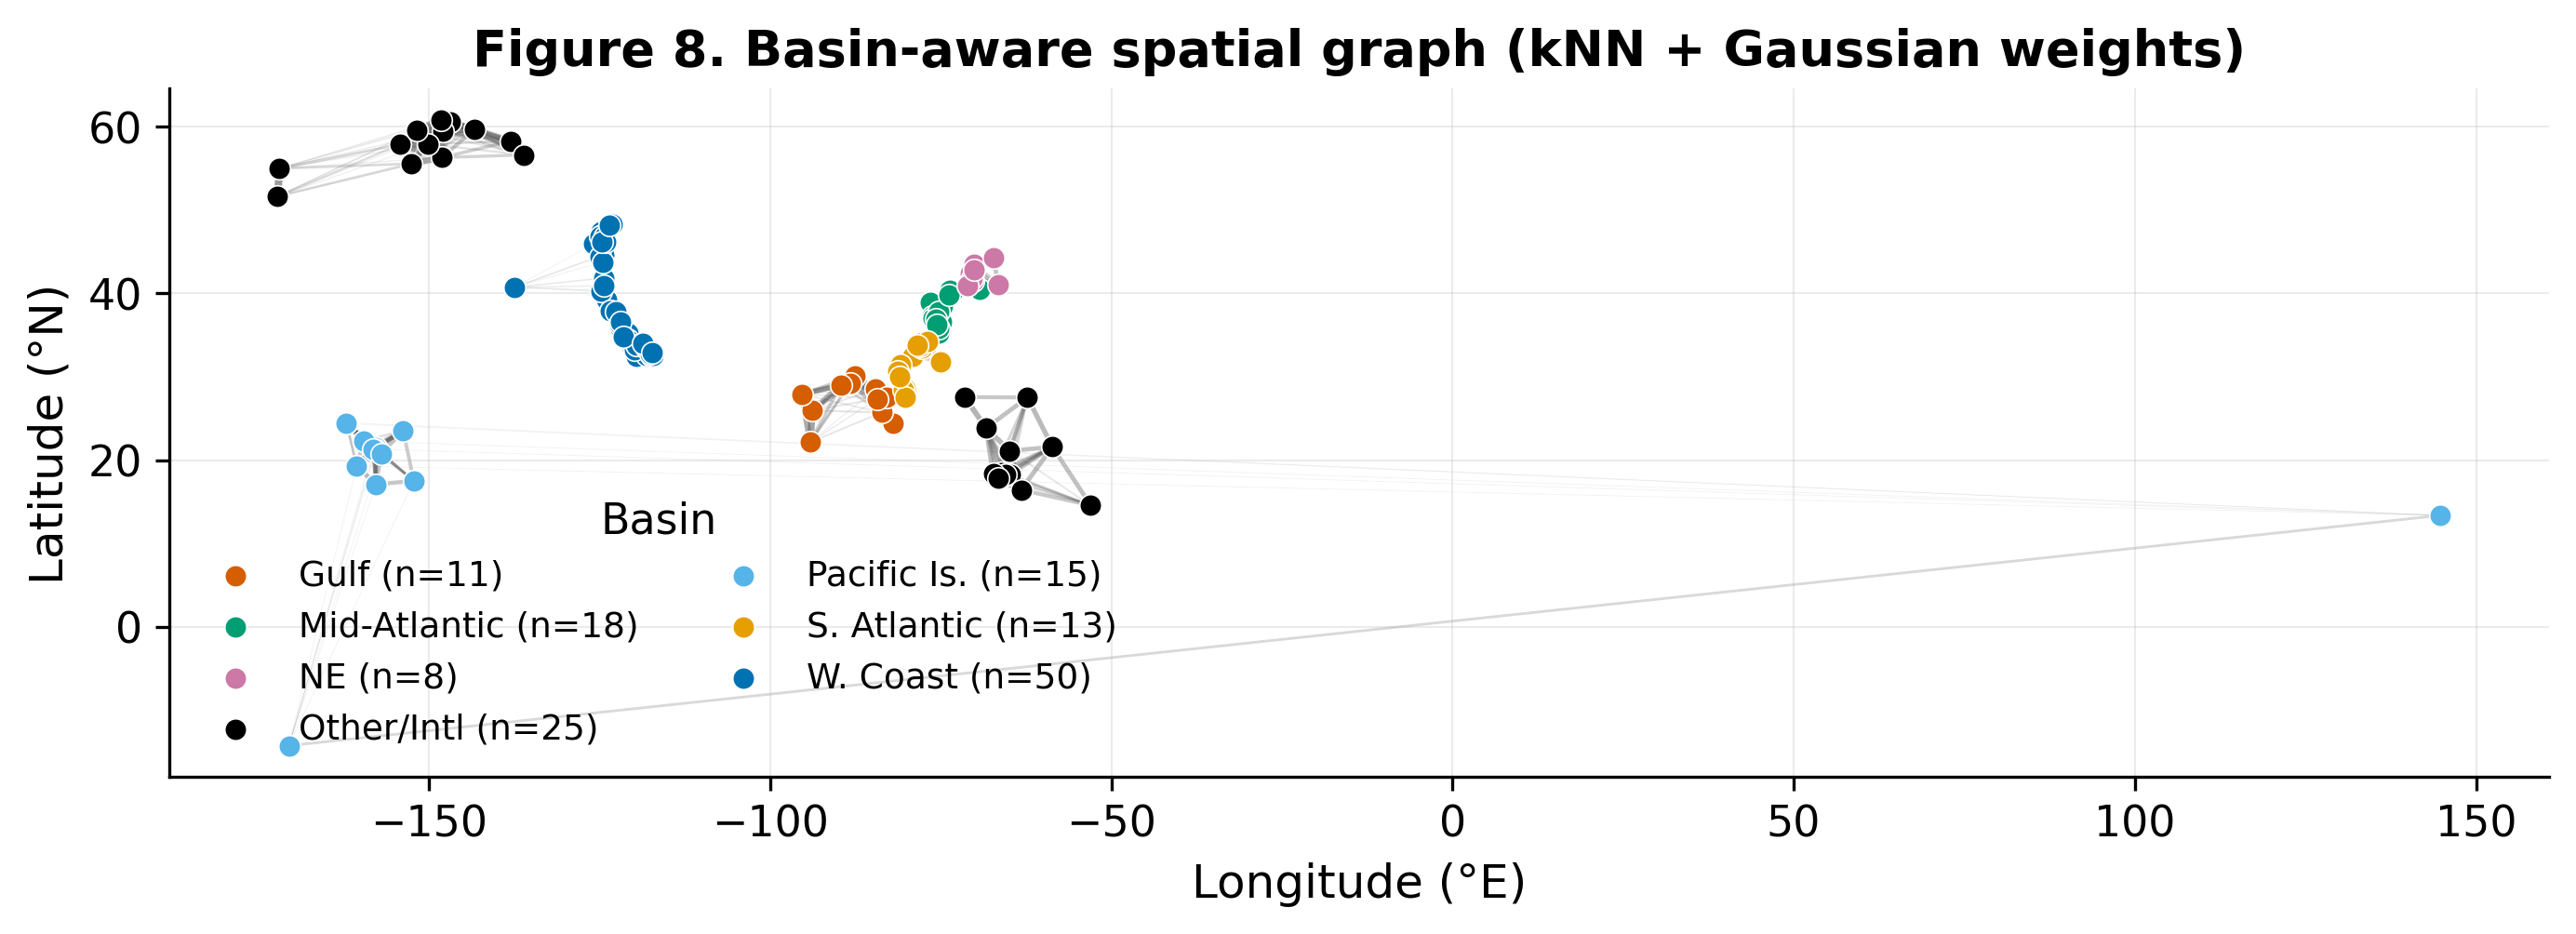
\includegraphics[width=\textwidth,height=0.72\textheight,keepaspectratio]{fig8_spatial_graph.png}
    \column{0.46\textwidth}
    \begin{itemize}\footnotesize
      \item Basin-aware $k$-NN ($k=8$), local self-tuning Gaussian weights.
      \item Documented coordinate corrections:
      \begin{itemize}
        \item[--] 51003 mislabeled near Japan $\rightarrow$ Western Hawaii.
        \item[--] 46006 (Station Papa) basin reassigned to W.\ Coast.
        \item[--] Florida Atlantic buoys re-tagged off Gulf.
      \end{itemize}
    \end{itemize}
  \end{columns}
  \take{The adjacency is auditable --- every correction is in \texttt{station\_corrections.yaml}.}
  \note{The corrections show we read the data, not just downloaded it. 51003 had a coordinate near Japan contradicting its name; 46006 sat just outside the West Coast box. Local self-tuning sigma prevents cross-scale underflow.}
\end{frame}

\begin{frame}{Methods, by paradigm}
  \begin{itemize}
    \item \textcolor{coltemporal}{\textbf{Classical / temporal}}: mean, forward-fill, linear interp\ldots
    \item \textcolor{colspatial}{\textbf{Spatial}}: inverse-distance weighting, spatial+temporal.
    \item \textcolor{coltemporal}{\textbf{Temporal deep}}: SAITS, BRITS.
    \item \textcolor{colgraph}{\textbf{Spatiotemporal graph}}: GRIN.
  \end{itemize}
  \vfill\plegend
  \note{Two independent temporal deep models (SAITS attention, BRITS recurrent) so that a failure on outage is architecture-independent. Only GRIN adds the adjacency.}
\end{frame}

\begin{frame}{Full imputation results (MAE, physical units)}
  \begin{center}
  \resizebox{\textwidth}{!}{%
  \begin{tabular}{l cc cc cc}
    \toprule
    & \multicolumn{2}{c}{Station-outage} & \multicolumn{2}{c}{MCAR-50\%} & \multicolumn{2}{c}{Block-50\%}\\
    \cmidrule(lr){2-3}\cmidrule(lr){4-5}\cmidrule(lr){6-7}
    Method & WVHT & APD & WVHT & APD & WVHT & APD\\
    \midrule
\textcolor{coltemporal}{Mean fill} & 0.458 & 0.955 & 0.476 & 0.997 & 0.445 & 0.968 \\
\textcolor{coltemporal}{Forward fill} & 0.637 & 1.303 & 0.111 & 0.306 & 0.702 & 1.410 \\
\textcolor{coltemporal}{Linear interp} & 0.637 & 1.303 & \textbf{0.074} & \textbf{0.211} & 0.557 & 1.186 \\
\textcolor{colspatial}{Spatial IDW} & 0.443 & 0.765 & 0.430 & 0.844 & 0.437 & 0.889 \\
\textcolor{colspatial}{Spatial+temporal} & 0.426 & 0.846 & 0.229 & 0.462 & 0.392 & 0.857 \\
\textcolor{coltemporal}{SAITS} & 0.743 & 1.694 & 0.086 & 0.214 & 0.598 & 0.809 \\
\textcolor{coltemporal}{BRITS} & 0.727 & 1.572 & 0.123 & 0.386 & 0.682 & 1.055 \\
\textcolor{colgraph}{GRIN} & \textbf{0.346$\pm$0.007} & \textbf{0.726$\pm$0.033} & 0.082$\pm$0.002 & 0.228$\pm$0.002 & \textbf{0.373$\pm$0.021} & \textbf{0.704$\pm$0.039} \\
    \bottomrule
  \end{tabular}}
  \end{center}
  \take{GRIN wins the structured regimes; linear interp wins only trivial MCAR.}\vspace{-1.2ex}\begin{center}\plegend\end{center}
  \note{GRIN mean +/- std over 3 model seeds. Bold is best per column. Note honestly that linear interp wins MCAR-50 -- isolated gaps are trivial -- but GRIN owns station-outage and block. Do not overclaim MCAR.}
\end{frame}

\begin{frame}{The dichotomy --- the hinge of the talk}
  \begin{center}\large
  \begin{tabular}{l cc}
    \toprule
    Method & Station-outage WVHT & MCAR-50 WVHT\\
    \midrule
    \onslide<2->{\textcolor{colspatial}{Spatial IDW}} & \onslide<2->{\textbf{0.443}} & \onslide<2->{0.430} \\
    \onslide<3->{\textcolor{coltemporal}{SAITS (temporal)}} & \onslide<3->{0.743} & \onslide<3->{\textbf{0.086}} \\
    \bottomrule
  \end{tabular}
  \end{center}
  \vfill
  \onslide<4->{\begin{center}\large\color{colgraph}\textbf{No single paradigm wins both.}\end{center}}
  \note{Build it slowly. Reveal IDW: spatial is fine on blackout, poor on scatter. Reveal SAITS: temporal is superb on scatter, worst on blackout. The crossover is the whole motivation. Then the punchline -- pause before advancing to GRIN.}
\end{frame}

\begin{frame}{GRIN wins both regimes}
  \begin{center}\large
  \begin{tabular}{l cc}
    \toprule
    & Station-outage WVHT & MCAR-50 WVHT\\
    \midrule
    \textcolor{colspatial}{Spatial IDW} & 0.443 & 0.430\\
    \textcolor{coltemporal}{SAITS} & 0.743 & 0.086\\
    \textcolor{colgraph}{\textbf{GRIN}} & \textbf{0.346$\pm$0.007} & \textbf{0.082}\\
    \bottomrule
  \end{tabular}
  \end{center}
  \take{First method strong in \emph{both} regimes --- the point of the whole imputation study.}
  \note{Station-outage WVHT 0.346 +/- 0.007 vs IDW 0.443 and SAITS 0.743. MCAR-50 competitive at 0.082. GRIN is the only row without a weak cell.}
\end{frame}

\begin{frame}{Mechanism: isolating the graph's contribution}
  \begin{itemize}
    \item GRIN and SAITS share the deep-learning machinery; they differ \emph{only} in the adjacency.
    \item Per-victim, station-by-station, on \texttt{station\_outage\_full}:
  \end{itemize}
  \begin{center}
  \begin{tabular}{l ccc}
    \toprule
    Target & GRIN & SAITS & Advantage\\
    \midrule
    WVHT (m, $n=$38) & 0.347 & 0.728 & \textbf{0.381}\\
    APD (s, $n=$33) & 0.767 & 1.628 & \textbf{0.861}\\
    \bottomrule
  \end{tabular}
  \end{center}
  \take{$\sim$0.381\,m WVHT and $\sim$0.861\,s APD --- attributable to the graph alone.}
  \note{Read from grin\_per\_victim\_outage.csv and saits\_per\_victim\_outage.csv, averaged over seeds then victims. Because the only difference is the adjacency, this difference is the causal contribution of message passing.}
\end{frame}

\begin{frame}{A reported null result: basin-aware vs.\ plain $k$-NN}
  \begin{center}\footnotesize
  \begin{tabular}{l l ccc c}
    \toprule
    Regime & Target & Basin-aware & Plain $k$-NN & Advantage & Exceeds noise\\
    \midrule
Station-outage & WVHT & 0.346$\pm$0.007 & 0.340$\pm$0.013 & -0.006 & no \\
Station-outage & APD & 0.726$\pm$0.033 & 0.745$\pm$0.052 & +0.018 & no \\
MCAR-50\% & WVHT & 0.082$\pm$0.002 & 0.083$\pm$0.002 & +0.001 & no \\
MCAR-50\% & APD & 0.228$\pm$0.002 & 0.228$\pm$0.002 & +0.000 & no \\
Block-50\% & WVHT & 0.373$\pm$0.021 & 0.363$\pm$0.015 & -0.010 & no \\
Block-50\% & APD & 0.704$\pm$0.039 & 0.716$\pm$0.032 & +0.012 & no \\
    \bottomrule
  \end{tabular}
  \end{center}
  \take{All 16/16 config$\times$target cells within model-seed noise --- a useful simplification.}
  \note{We volunteer this null. The Gaussian kernel already suppresses cross-basin edges, so hard basin masking adds nothing. Framing it as a simplification, not a failure, is the honest and stronger move. Full 16-cell grid is in backup.}
\end{frame}

\begin{frame}{Connectivity vs.\ recovery: directional, underpowered}
  \begin{center}\footnotesize
  \begin{tabular}{l l ccc}
    \toprule
    Target & Connectivity measure & Raw & Normalized & Advantage\\
    \midrule
WVHT & degree & -0.36$^{*}$ & -0.53$^{*}$ & +0.21 \\
WVHT & neighbour dist. & +0.59$^{*}$ & +0.29 & -0.19 \\
WVHT & edge-weight sum & -0.46$^{*}$ & -0.52$^{*}$ & +0.16 \\
APD & degree & +0.26 & -0.35$^{*}$ & +0.16 \\
APD & neighbour dist. & -0.46$^{*}$ & -0.01 & -0.47$^{*}$ \\
APD & edge-weight sum & +0.40$^{*}$ & -0.20 & +0.38$^{*}$ \\
    \bottomrule
  \end{tabular}\\[0.5ex]
  {\scriptsize $^{*}p<0.05$; Spearman $\rho$. $n=$38 (WVHT), 33 (APD).}
  \end{center}
  \take{Signs match the hypothesis, several are significant --- but $n\approx$38 is underpowered. We do not overclaim.}
  \note{Better-connected stations tend to lower normalized error (negative rho). State plainly this is suggestive, not a law -- the sample is the 38 outage victims. Do not let anyone walk away thinking this is a confirmed scaling relationship.}
\end{frame}

% ##################### PART IV #####################
\section{Part IV \textperiodcentered\ Forecasting}

\begin{frame}{Forecasting setup}
  \begin{itemize}
    \item Input window 24\,h; horizons \textbf{12\,h} and \textbf{24\,h}.
    \item 1\,h dropped: persistence is saturated there (see horizon sweep, fig.\ 10).
    \item Baselines: \textcolor{coltemporal}{persistence}, \textcolor{coltemporal}{AR(24)}; model: \textcolor{colgraph}{Graph WaveNet}.
  \end{itemize}
  \take{We report where a learned model actually earns its keep: the multi-hour horizons.}
  \note{Being honest that 1h is a persistence regime is a credibility move -- we are not cherry-picking horizons that flatter the model. AR(24) is a strong per-station linear competitor.}
\end{frame}

\begin{frame}{Leakage control at test time}
  \begin{itemize}
    \item \textbf{Train:} model sees a GRIN-completed tensor (bidirectional fill, training period only).
    \item \textbf{Test:} neighbour inputs use \emph{causal forward-fill only} --- never the bidirectional GRIN values.
    \item Scored only at origins where the full window and the target at $t+h$ are genuinely observed.
  \end{itemize}
  \take{No future information --- and no bidirectional imputation --- ever enters a test forecast.}
  \note{This is the other question magnet. The subtlety: we may train on GRIN-completed data (past-and-future within the training years) but at test we must not, so test inputs are causal forward-fill. Give this its own breath.}
\end{frame}

\begin{frame}{Forecast results (MAE; skill vs.\ persistence)}
  \begin{center}
  \resizebox{\textwidth}{!}{%
  \begin{tabular}{l cc cc}
    \toprule
    & \multicolumn{2}{c}{WVHT (m)} & \multicolumn{2}{c}{APD (s)}\\
    \cmidrule(lr){2-3}\cmidrule(lr){4-5}
    Method & $h{=}12$ & $h{=}24$ & $h{=}12$ & $h{=}24$\\
    \midrule
\textcolor{coltemporal}{Persistence} & 0.296 & 0.416 & 0.724 & 0.884 \\
\textcolor{coltemporal}{AR(24)} & 0.280 (+0.054) & 0.378 (+0.090) & 0.654 (+0.096) & 0.789 (+0.107) \\
\textcolor{colgraph}{GraphWaveNet} & 0.249 (+0.158) & 0.347 (+0.166) & 0.607 (+0.161) & 0.745 (+0.157) \\
    \bottomrule
  \end{tabular}}
  \end{center}
  \take{Graph WaveNet $\sim$16\% skill throughout --- AR(24) only 0.054--0.107.}
  \note{GWN skill: WVHT +0.158/+0.166, APD +0.161/+0.157. AR(24) sits at 0.054-0.107. Roughly triple at the short end -- that is the "3x" claim from the thesis slide. Persistence is the zero reference by construction.}
\end{frame}

\begin{frame}{Skill grows with horizon}
  \begin{center}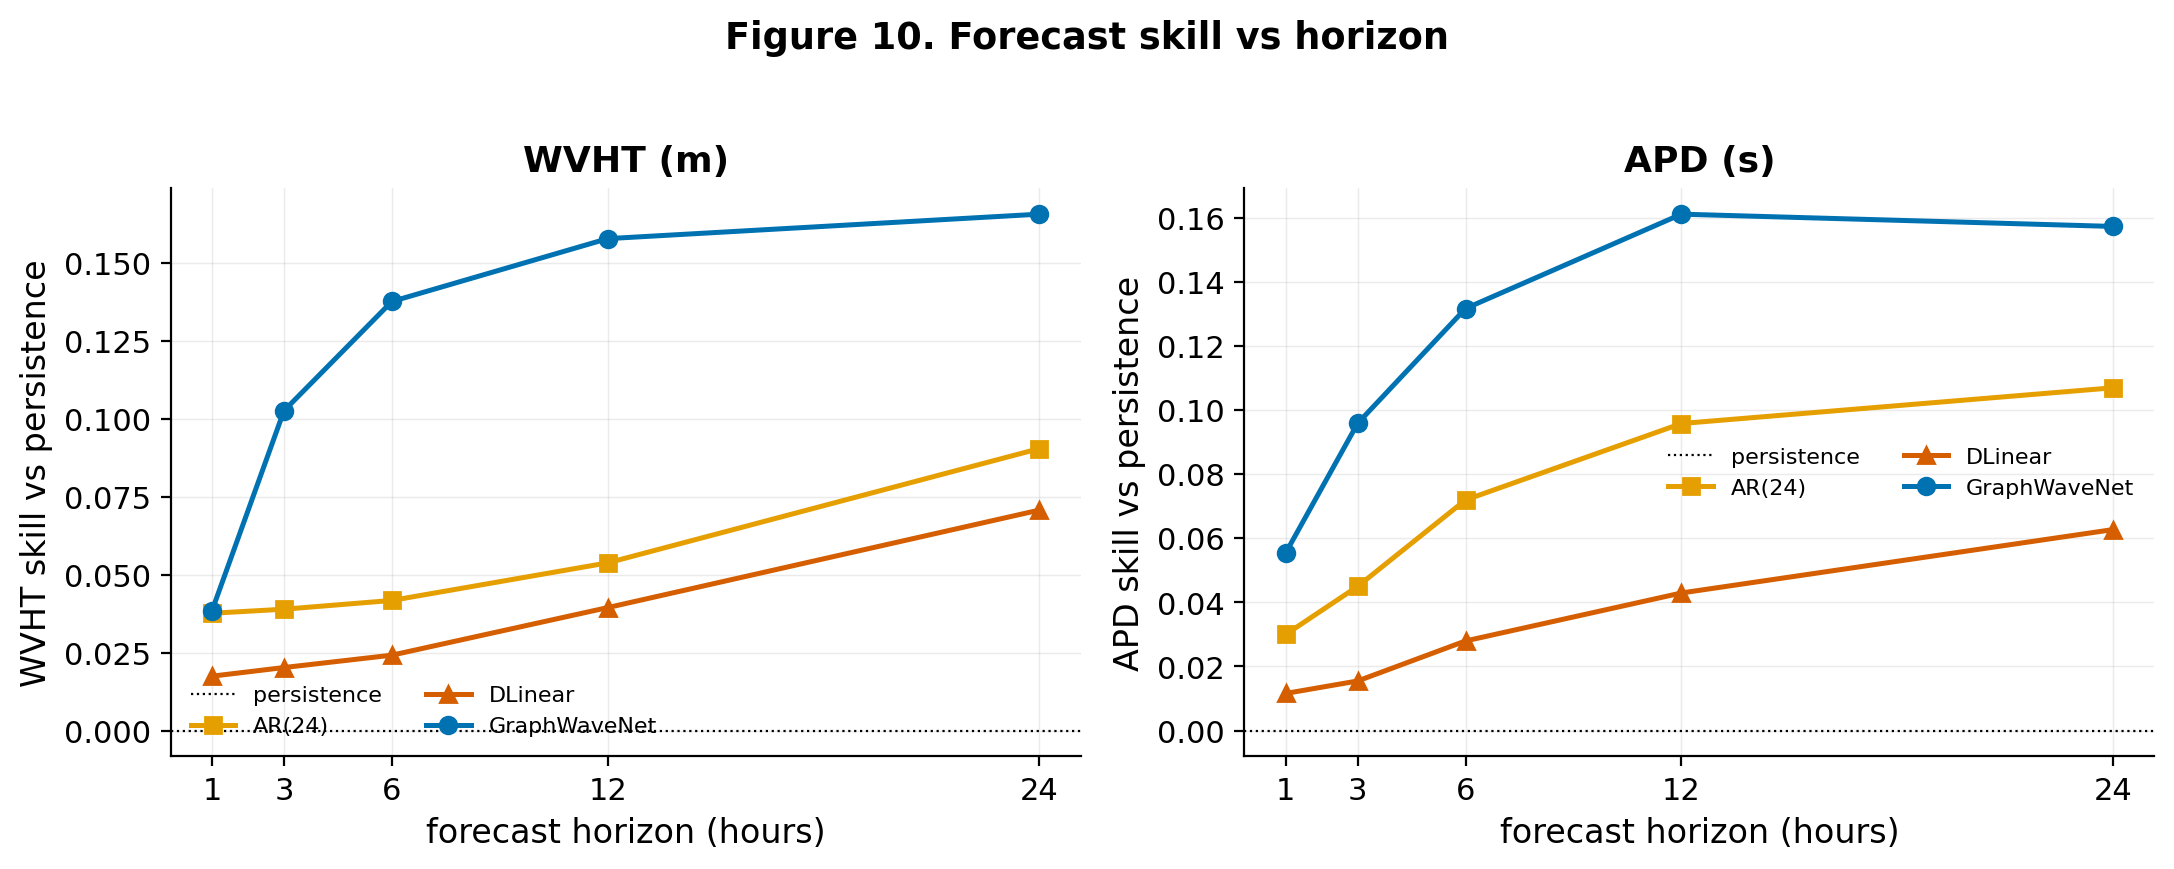
\includegraphics[width=\textwidth,height=0.66\textheight,keepaspectratio]{fig10_horizon_skill.png}\end{center}
  \take{Persistence saturates early; the graph opens the widest gap at 12--24\,h.}
  \note{The gap between the learned models and persistence widens with horizon -- exactly where an operator needs the forecast. This justifies dropping 1h.}
\end{frame}

\begin{frame}{The parallel: two tasks, one story}
  \begin{center}
  \resizebox{\textwidth}{!}{%
  \begin{tabular}{l l l l}
    \toprule
    Task & Metric & Single-paradigm floor & Spatiotemporal graph\\
    \midrule
Imputation & station-outage WVHT MAE & \textcolor{colspatial}{Spatial IDW} 0.443, \textcolor{coltemporal}{SAITS} 0.743 & \textbf{\textcolor{colgraph}{GRIN} 0.346} \\
Forecasting & 24h WVHT skill & \textcolor{coltemporal}{AR(24)} +0.090 & \textbf{\textcolor{colgraph}{GraphWaveNet} +0.166} \\
    \bottomrule
  \end{tabular}}
  \end{center}
  \take{Two independent tasks, one shape: a single-paradigm floor, beaten by the graph.}
  \note{This is the rhyme of the talk. Same shape twice: temporal or spatial alone hits a floor; the spatiotemporal graph clears it. Two independent tasks, one mechanism.}
\end{frame}

% ##################### PART V #####################
\section{Part V \textperiodcentered\ Wave Energy}

\begin{frame}{The physics}
  \begin{center}\large
  $P \;=\; \dfrac{\rho g^{2}}{64\pi}\, H_{m0}^{2}\, T_e \;\approx\; 0.49\, H^{2}\, T_e \quad$ (kW/m)
  \end{center}
  \begin{itemize}
    \item Power scales with the \textbf{square} of wave height and \emph{linearly} with energy period.
    \item So a better height forecast earns a \emph{squared} payoff in power.
  \end{itemize}
  \note{Set up the H-squared nonlinearity here so the amplification on the results slide is expected, not a surprise. Flux formula anchored to Guillou 2020.}
\end{frame}

\begin{frame}{APD $\rightarrow T_e$: a documented, invariance-safe conversion}
  \begin{itemize}
    \item NDBC reports APD, not the energy period $T_e$. We set $T_e=\alpha\cdot\text{APD}$, $\alpha=1.12$ (config-exposed).
    \item $\alpha$ is an \emph{empirical} wave-period ratio (Cahill \& Lewis 2014) --- their paper argues \emph{against} the theoretical JONSWAP ratios.
    \item Flux formula anchored to Guillou (2020, \emph{Renewable Energy}, NDBC buoys).
    \item \textbf{Invariance:} $\alpha$ scales every method identically $\Rightarrow$ rankings and skill are unchanged.
  \end{itemize}
  \note{Two precision points the co-authors will check: (1) do NOT call 1.12 the JONSWAP ratio -- Cahill and Lewis empirically dispute the theoretical ratios; call it an empirical ratio consistent with their measurements. (2) The invariance argument means our comparative claims survive any alpha in the cited range.}
\end{frame}

\begin{frame}{Energy results: the advantage amplifies}
  \begin{center}
  \begin{tabular}{l cc}
    \toprule
    Method & $h{=}12$ & $h{=}24$\\
    \midrule
\textcolor{coltemporal}{Persistence} & 5.468 & 7.691 \\
\textcolor{coltemporal}{AR(24)} & 4.863 (+0.111) & 6.434 (+0.164) \\
\textcolor{colgraph}{GraphWaveNet} & 4.284 (+0.217) & 5.882 (+0.235) \\
    \bottomrule
  \end{tabular}\\[0.5ex]
  {\footnotesize MAE in kW/m; skill vs.\ persistence in parentheses.}
  \end{center}
  \take{Graph skill +0.217/+0.235 --- wider than its height skill: the $H^2$ nonlinearity amplifies it.}
  \note{GWN energy skill exceeds its own height skill because power squares height, where the graph is strongest. AR(24) sits at +0.111/+0.164. This is the applied payoff -- the number an operator cares about is where the graph wins by the most.}
\end{frame}

% ##################### CLOSING #####################
\section{Contributions \& Limitations}

\begin{frame}{Contributions}
  \begin{enumerate}
    \item A pre-registered, leakage-safe benchmark separating scattered from structured missingness (slides 10--13).
    \item The first imputer strong in \emph{both} regimes --- GRIN --- with the graph's contribution isolated per victim (slides 18--20).
    \item The graph advantage carried through forecasting to \emph{wave power}, amplified by the $H^2$ nonlinearity (slides 25--30).
  \end{enumerate}
  \note{Three claims, each tied to slide numbers so the committee can jump back. Lead with the benchmark (methodology), then the dichotomy result, then the applied payoff.}
\end{frame}

\begin{frame}{Limitations --- volunteered}
  \begin{enumerate}\small
    \item Connectivity analysis underpowered ($n\approx$38).
    \item Deep-water flux assumption breaks nearshore (Wang, Duan \& Dong 2016).
    \item APD~$\approx T_{02}$ assumption pending co-author sign-off.
    \item Basin-aware graph adds nothing over plain $k$-NN.
    \item Single test year (2025); not yet multi-year cross-validated.
  \end{enumerate}
  \note{Volunteering these disarms the interrogation. Each has a planned response: (1) more victims, (3) spectral check with co-authors, (5) roll the split across years. Say we already know these, we are not hiding them.}
\end{frame}

\begin{frame}{Reproducibility}
  \begin{itemize}\small
    \item Pinned environment; \texttt{EVALUATION.md} pre-registered; every step committed.
    \item GRIN seeded, checkpointed, 3-seed aggregated.
    \item An uncapped 100-epoch run scored marginally better (\textbf{[VERIFY]}\,$\approx$0.331) but was \emph{discarded} for irreproducibility --- a deliberate trade.
  \end{itemize}
  \take{We chose a reproducible 0.346 over an unrepeatable 0.331.}
  \note{The discarded-run story is a credibility asset: we had a better number and threw it away because we could not reproduce it. That 0.331 is not in a committed CSV -- flagged VERIFY. State the trade explicitly.}
\end{frame}

\begin{frame}[plain]
  \vfill\begin{center}
  {\color{colgraph}\Large\bfseries Thank you}\\[1ex]
  {\large Questions}
  \end{center}\vfill
  \note{Likely questions: why hide known values (slide 13), leakage at test (slide 24), alpha invariance (slide 29), connectivity power (slide 22). Backup slides cover all four.}
\end{frame}

% ##################### BACKUP #####################
\appendix
\section{Backup}

\begin{frame}{Backup: full classical baselines (WVHT MAE, all rates)}
  \begin{center}\scriptsize
  \begin{tabular}{l ccc ccc c}
    \toprule
    Method & MCAR-10 & MCAR-30 & MCAR-50 & Block-10 & Block-30 & Block-50 & Outage\\
    \midrule
\textcolor{coltemporal}{Mean fill} & 0.476 & 0.476 & 0.476 & 0.474 & 0.451 & 0.445 & 0.458 \\
\textcolor{coltemporal}{Forward fill} & 0.088 & 0.097 & 0.111 & 0.599 & 0.628 & 0.702 & 0.637 \\
\textcolor{coltemporal}{Linear interp} & 0.065 & 0.068 & 0.074 & 0.520 & 0.504 & 0.557 & 0.637 \\
\textcolor{colspatial}{Spatial IDW} & 0.376 & 0.399 & 0.430 & 0.366 & 0.381 & 0.437 & 0.443 \\
\textcolor{colspatial}{Spatial+temporal} & 0.202 & 0.213 & 0.229 & 0.351 & 0.354 & 0.392 & 0.426 \\
    \bottomrule
  \end{tabular}
  \end{center}
\end{frame}

\begin{frame}{Backup: BRITS across all configs (MAE)}
  \begin{center}\footnotesize
  \begin{tabular}{l cc}
    \toprule
    Config & WVHT & APD\\
    \midrule
MCAR-10\% & 0.083 & 0.242 \\
MCAR-30\% & 0.097 & 0.301 \\
MCAR-50\% & 0.123 & 0.386 \\
Block-10\% & 0.809 & 0.973 \\
Block-30\% & 0.738 & 1.025 \\
Block-50\% & 0.682 & 1.055 \\
Outage-720h & 0.908 & 2.167 \\
Outage-full & 0.727 & 1.572 \\
    \bottomrule
  \end{tabular}\\[0.5ex]
  {\footnotesize Second temporal architecture; like SAITS it fails the outage regime --- an architecture-independent result.}
  \end{center}
\end{frame}

\begin{frame}{Backup: per-victim GRIN$-$SAITS advantage distribution}
  \begin{center}\footnotesize
  \begin{tabular}{l c ccc c c}
    \toprule
    Target & $n$ & min & median & mean & max & \#\,GRIN better\\
    \midrule
WVHT & 38 & +0.014 & +0.318 & +0.381 & +0.752 & 38/38 \\
APD & 33 & +0.070 & +0.813 & +0.861 & +2.081 & 33/33 \\
    \bottomrule
  \end{tabular}
  \end{center}
\end{frame}

\begin{frame}{Backup: full 16-cell ablation grid}
  \begin{center}\scriptsize
  \begin{tabular}{l l cc c c c}
    \toprule
    Config & Target & Basin & Plain & Advantage & Seed SD & Exceeds noise\\
    \midrule
MCAR-10\% & WVHT & 0.066 & 0.066 & +0.000 & 0.001 & no \\
MCAR-10\% & APD & 0.181 & 0.181 & -0.000 & 0.001 & no \\
MCAR-30\% & WVHT & 0.071 & 0.072 & +0.000 & 0.002 & no \\
MCAR-30\% & APD & 0.198 & 0.198 & -0.000 & 0.002 & no \\
MCAR-50\% & WVHT & 0.082 & 0.083 & +0.001 & 0.003 & no \\
MCAR-50\% & APD & 0.228 & 0.228 & +0.000 & 0.003 & no \\
Block-10\% & WVHT & 0.333 & 0.322 & -0.010 & 0.044 & no \\
Block-10\% & APD & 0.615 & 0.622 & +0.007 & 0.019 & no \\
Block-30\% & WVHT & 0.341 & 0.330 & -0.012 & 0.039 & no \\
Block-30\% & APD & 0.640 & 0.649 & +0.008 & 0.032 & no \\
Block-50\% & WVHT & 0.373 & 0.363 & -0.010 & 0.026 & no \\
Block-50\% & APD & 0.704 & 0.716 & +0.012 & 0.050 & no \\
Outage-720h & WVHT & 0.473 & 0.474 & +0.002 & 0.055 & no \\
Outage-720h & APD & 0.912 & 0.940 & +0.028 & 0.118 & no \\
Outage-full & WVHT & 0.346 & 0.340 & -0.006 & 0.015 & no \\
Outage-full & APD & 0.726 & 0.745 & +0.018 & 0.062 & no \\
    \bottomrule
  \end{tabular}
  \end{center}
\end{frame}

\begin{frame}{Backup: additional EDA figures}
  \begin{columns}
    \column{0.5\textwidth}\centering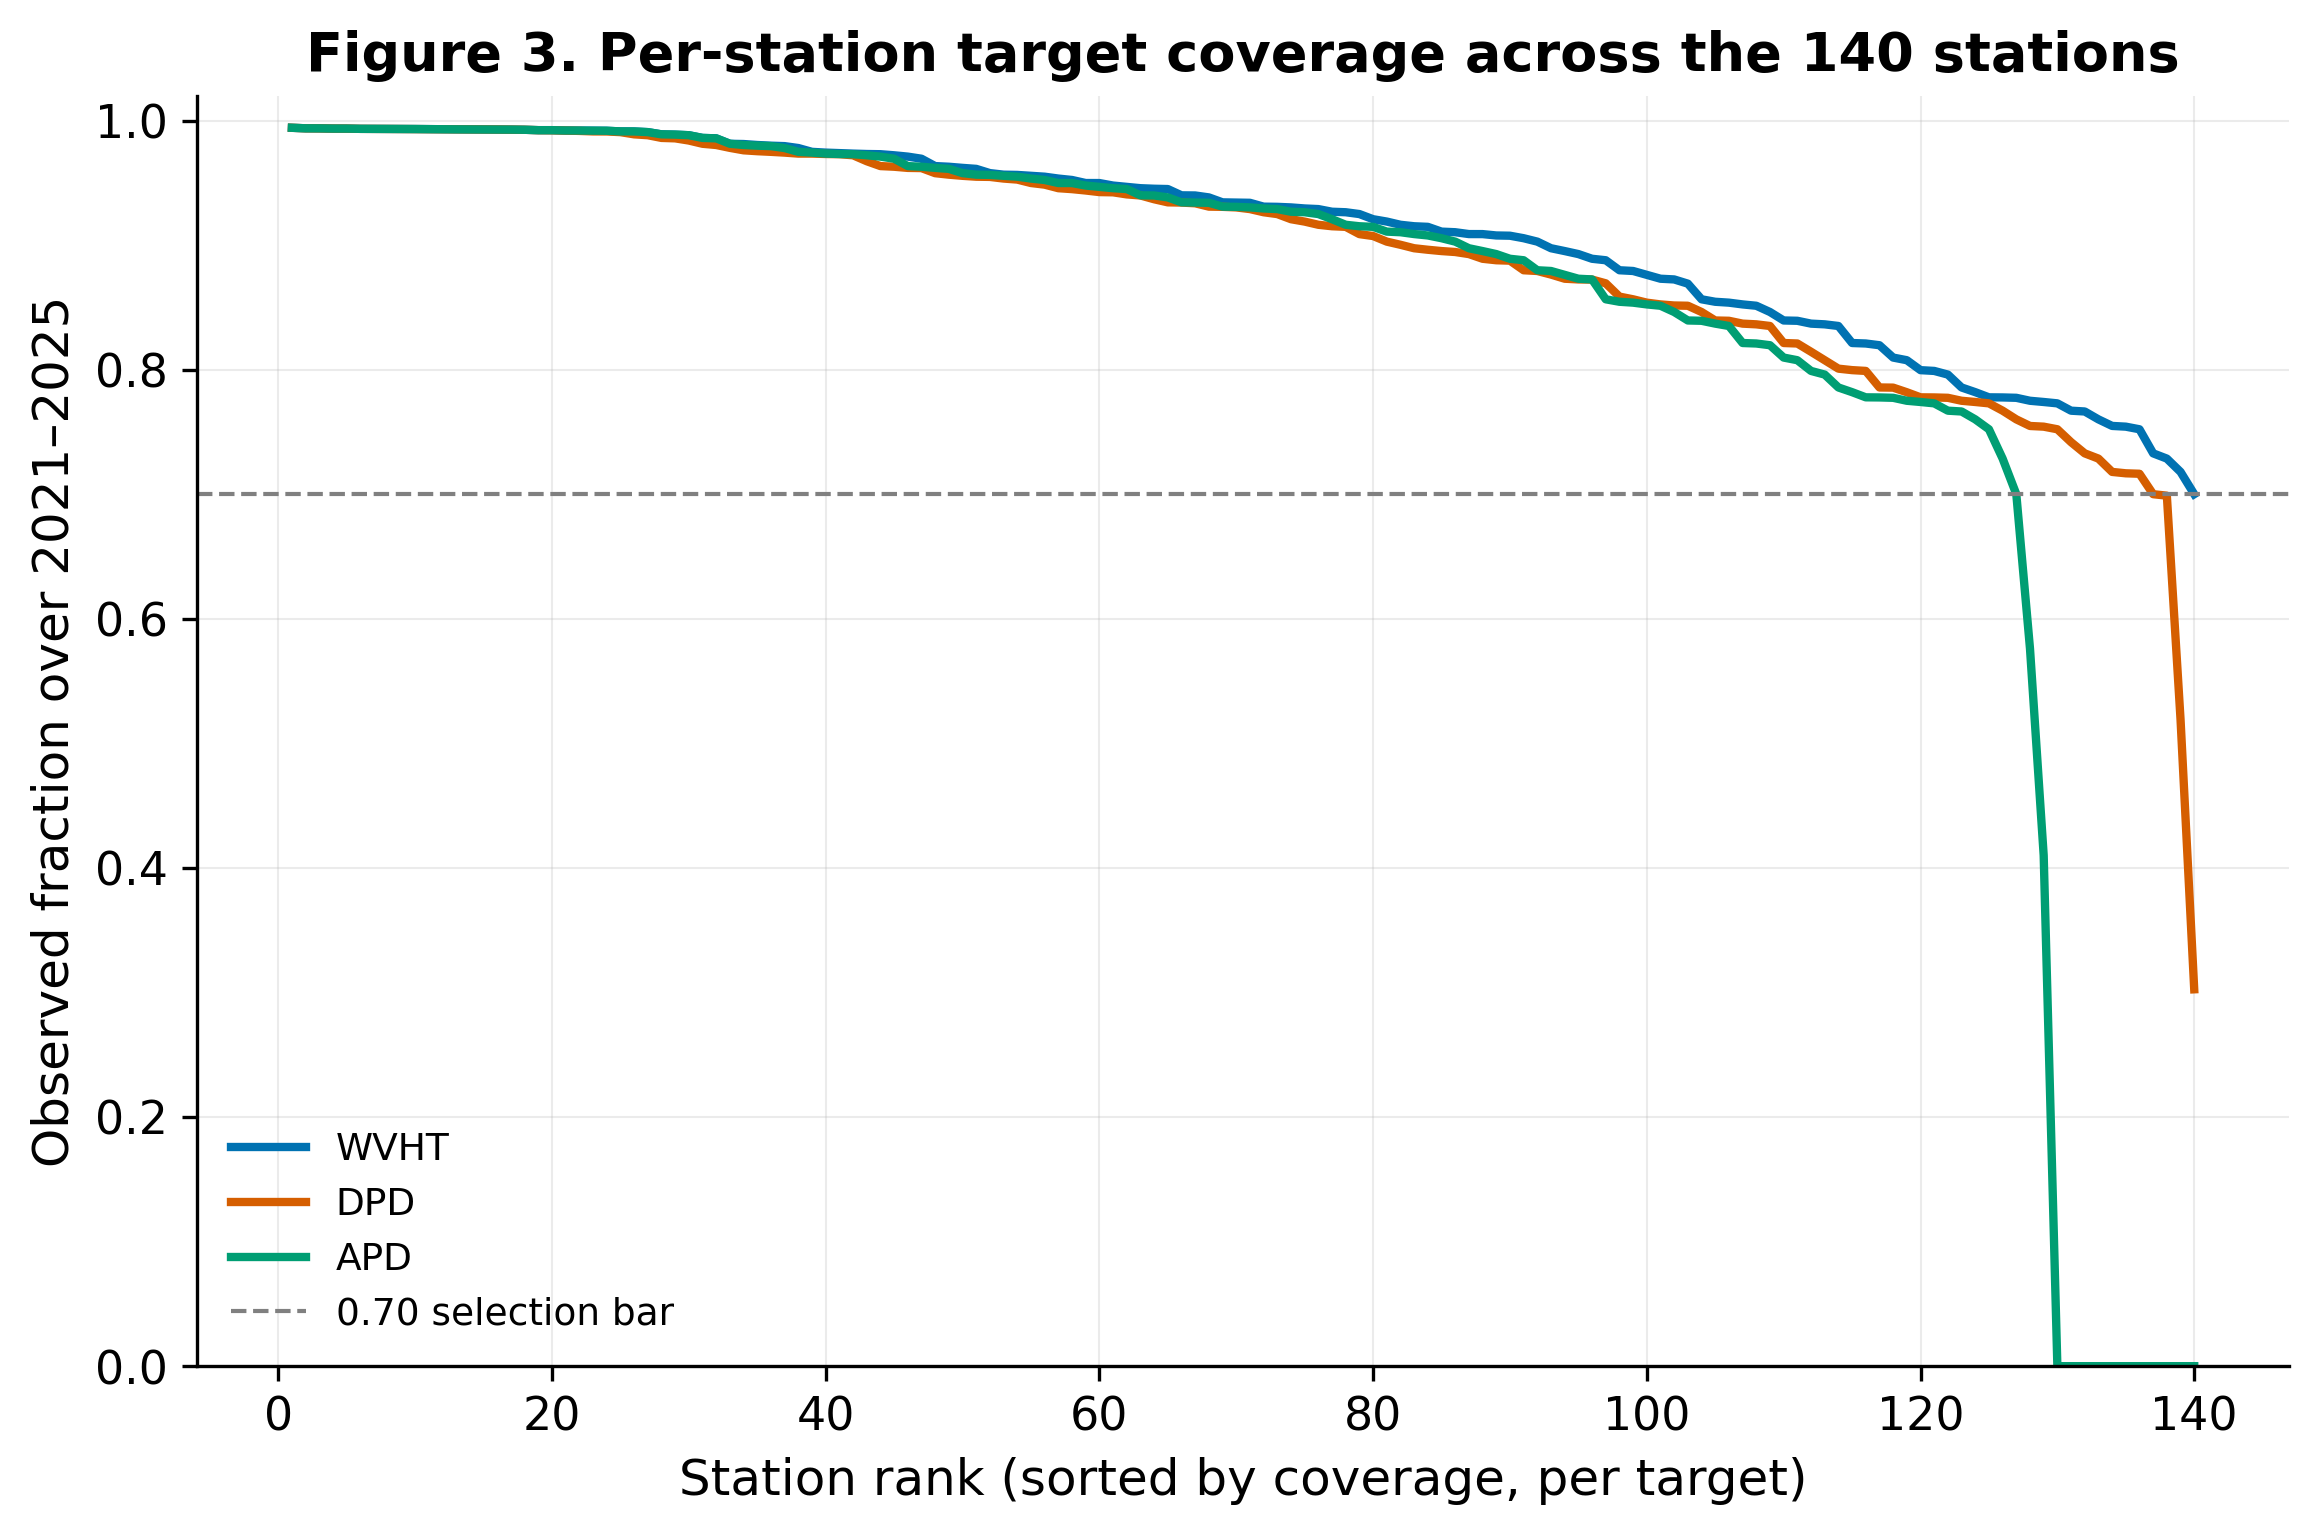
\includegraphics[width=\textwidth,height=0.72\textheight,keepaspectratio]{fig3_coverage_dist.png}
    \column{0.5\textwidth}\centering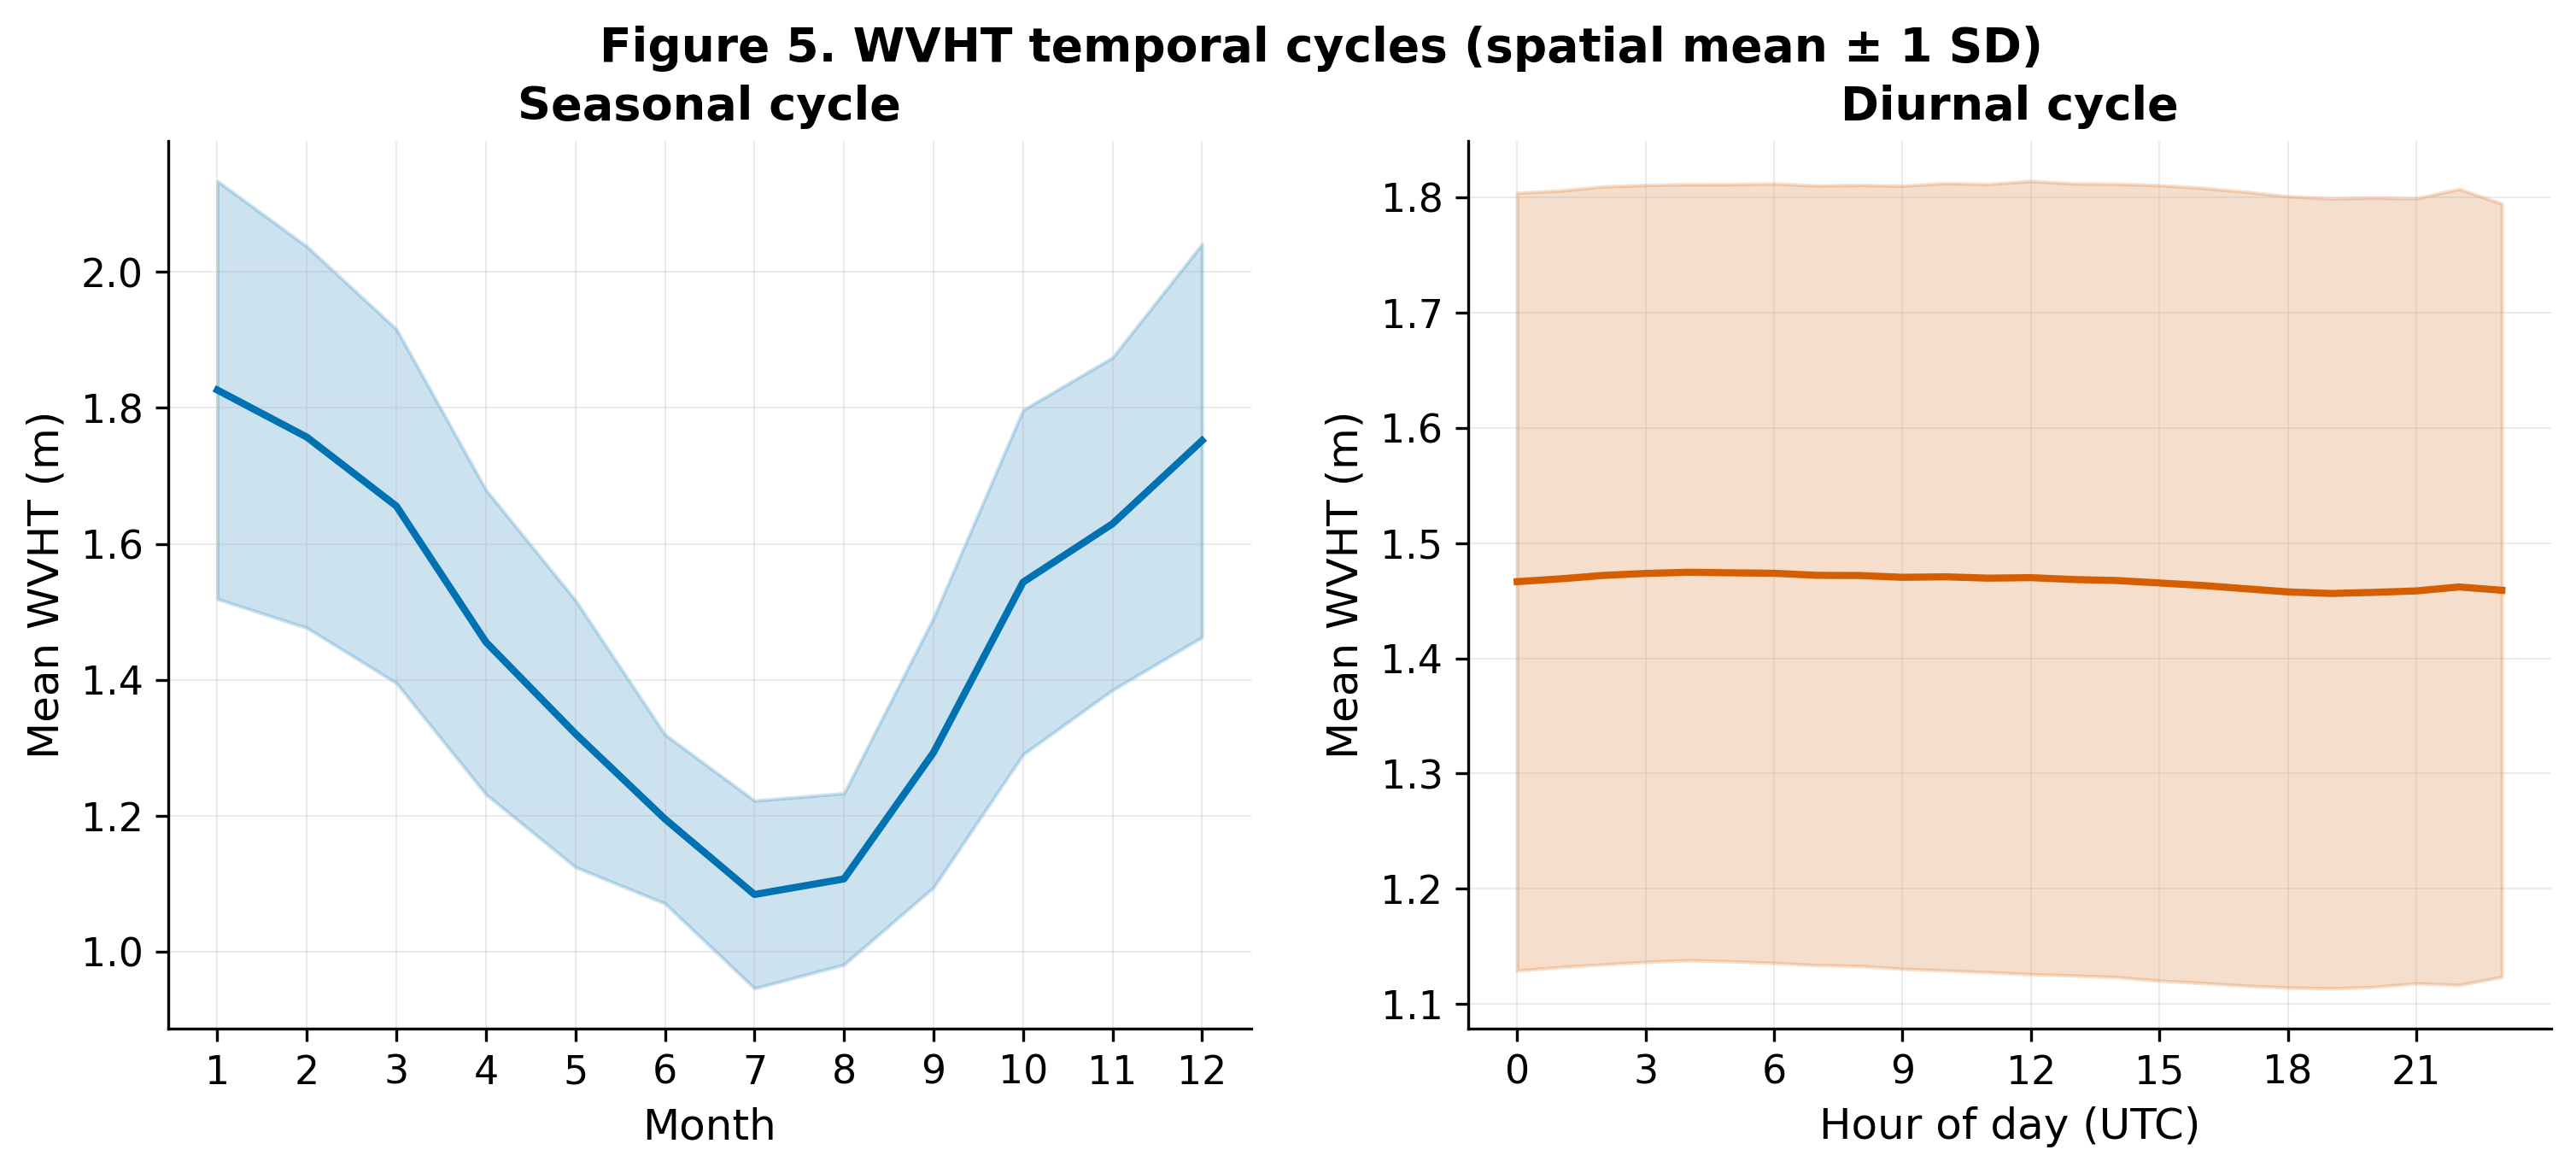
\includegraphics[width=\textwidth,height=0.72\textheight,keepaspectratio]{fig5_temporal_cycles.png}
  \end{columns}
\end{frame}

\begin{frame}{Backup: distributions and connectivity}
  \begin{columns}
    \column{0.5\textwidth}\centering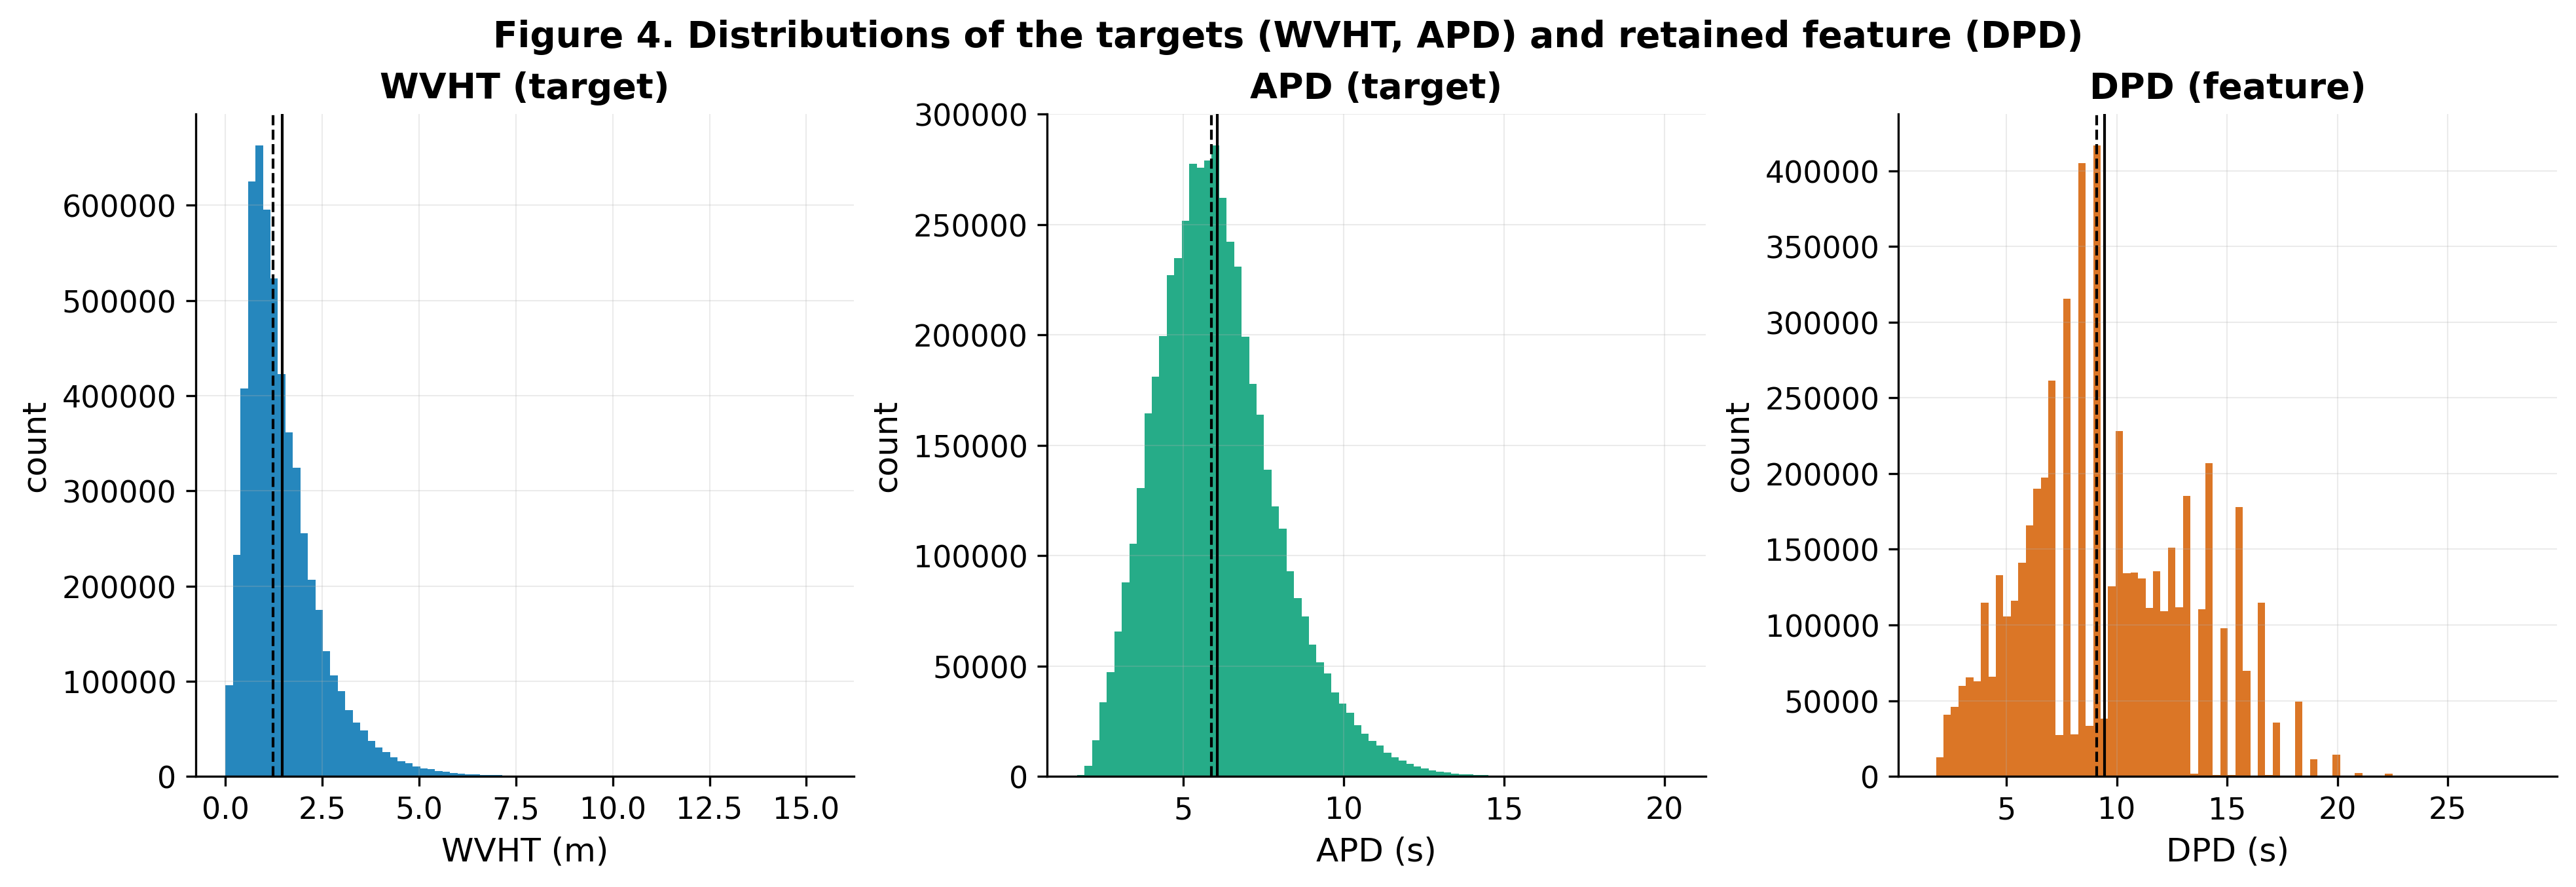
\includegraphics[width=\textwidth,height=0.72\textheight,keepaspectratio]{fig4_target_dists.png}
    \column{0.5\textwidth}\centering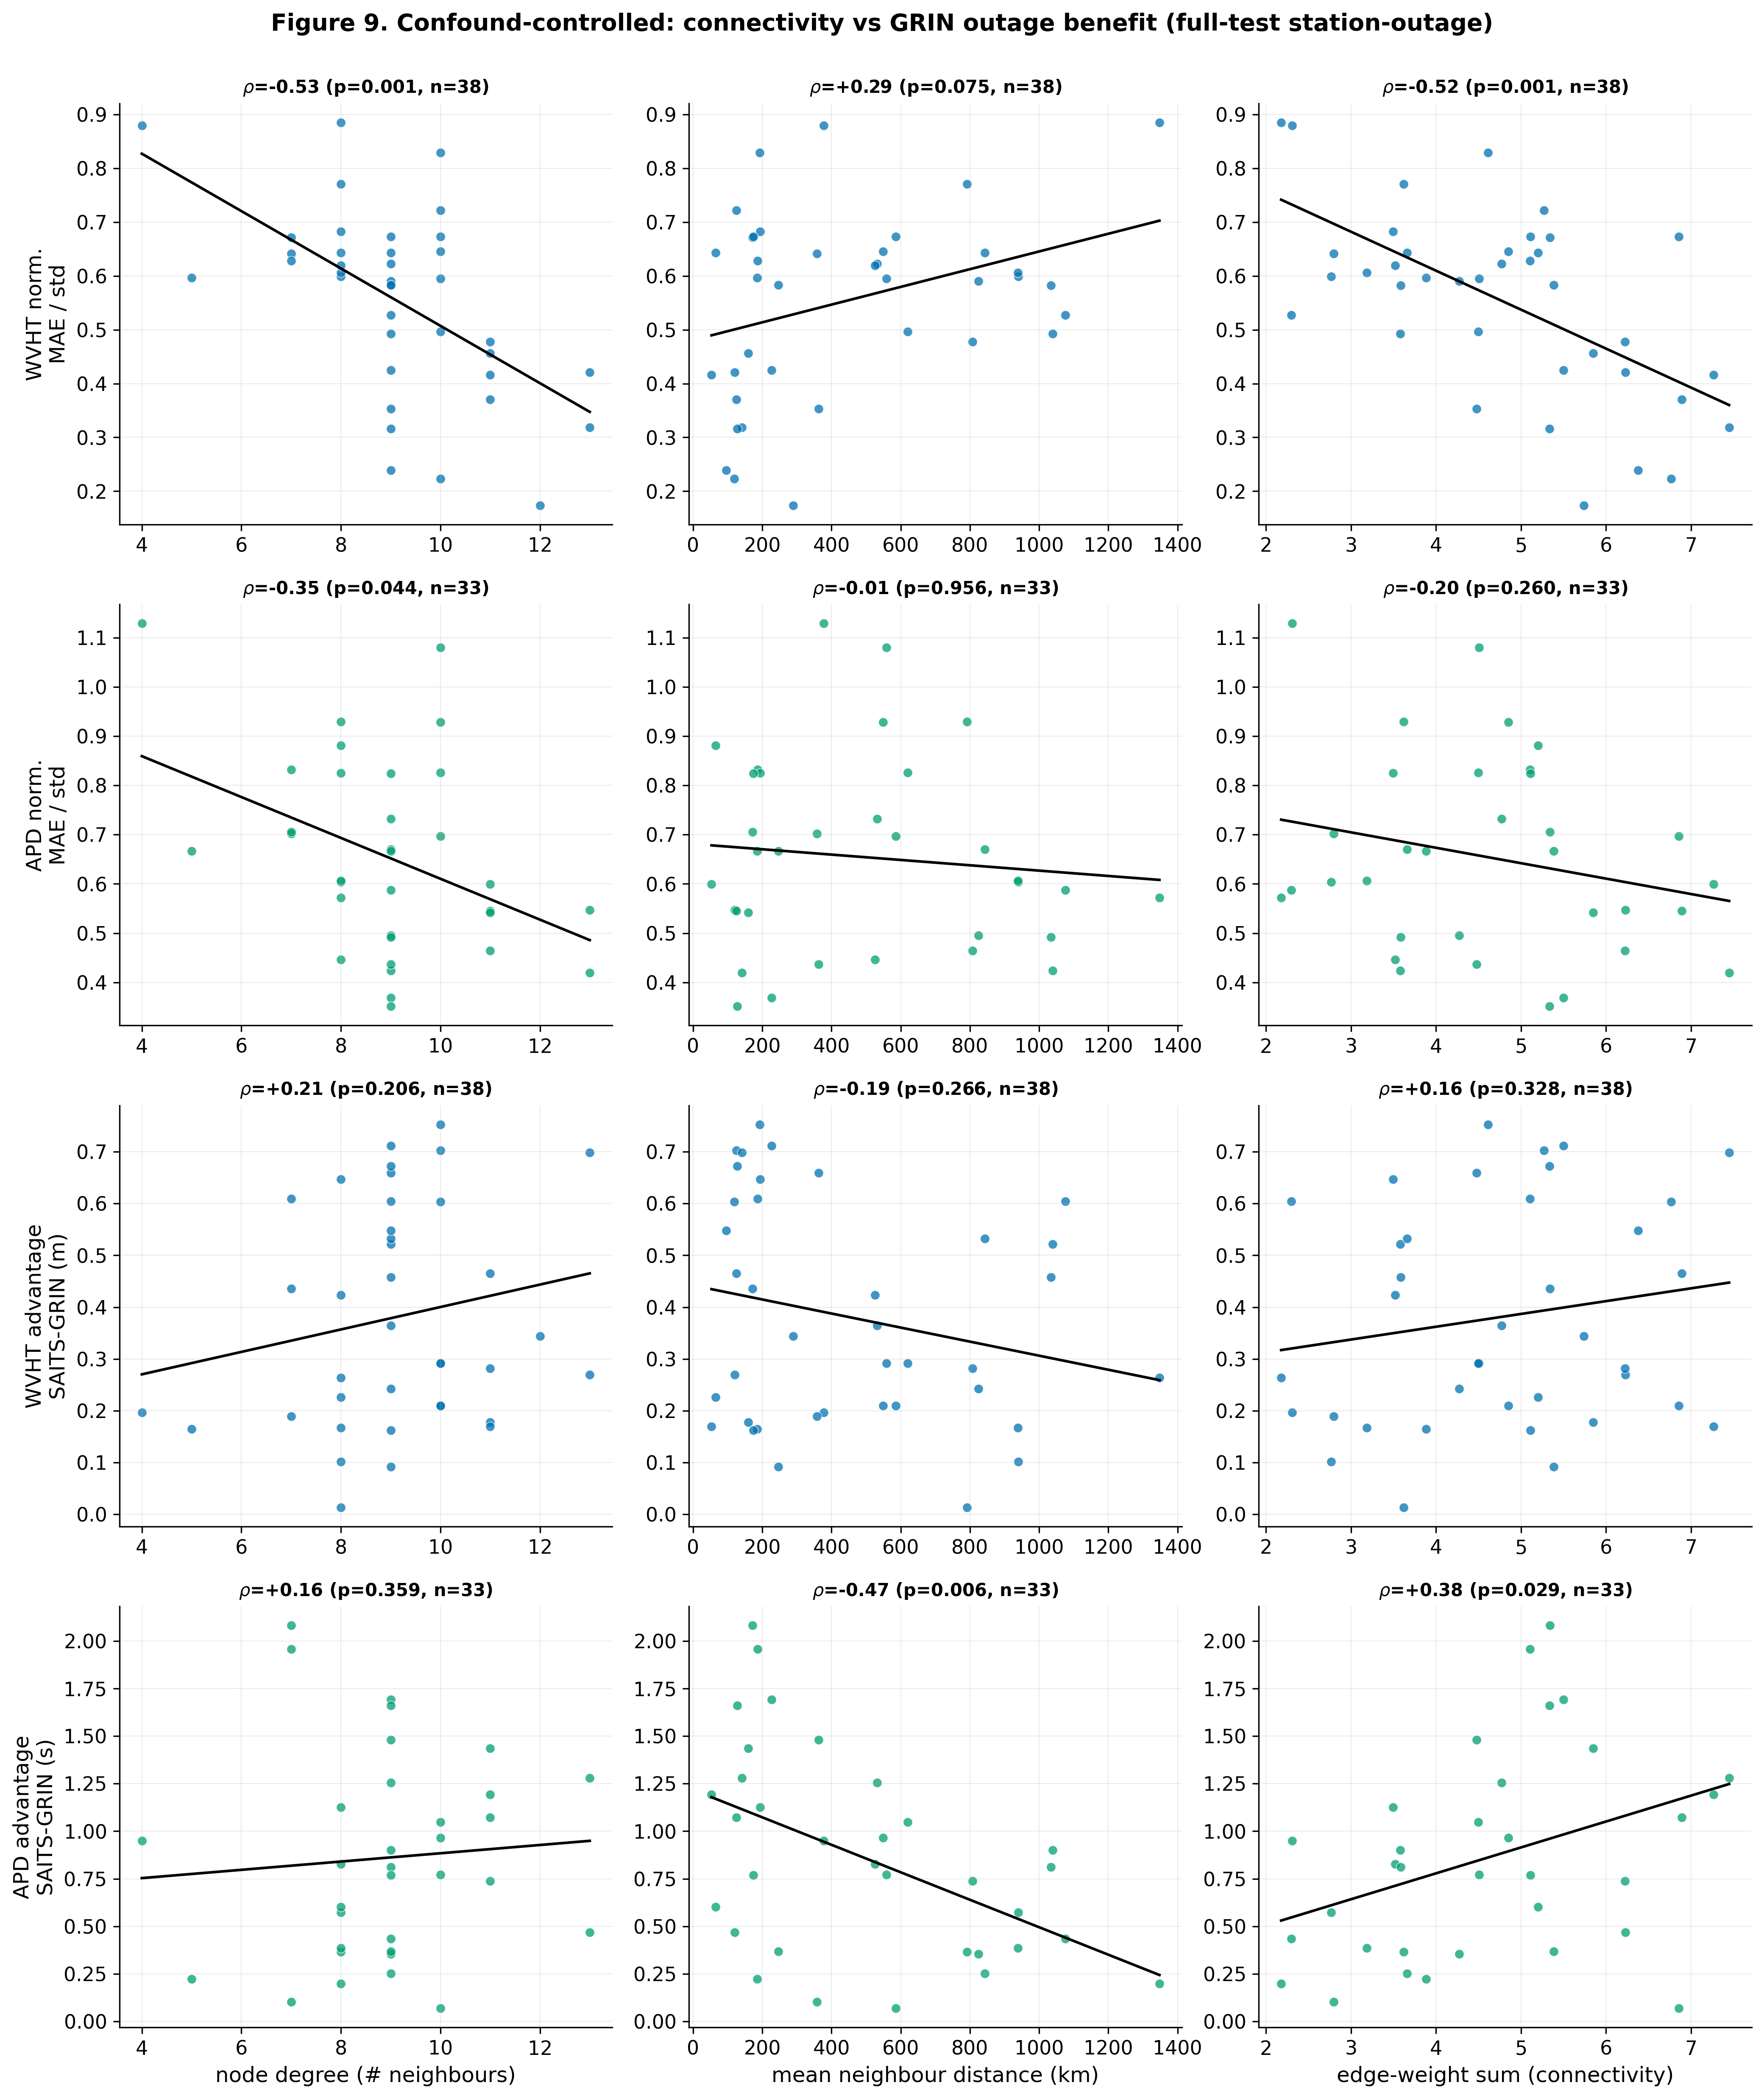
\includegraphics[width=\textwidth,height=0.72\textheight,keepaspectratio]{fig9_connectivity_recovery.png}
  \end{columns}
\end{frame}

\begin{frame}{Backup: energy forecast skill}
  \begin{center}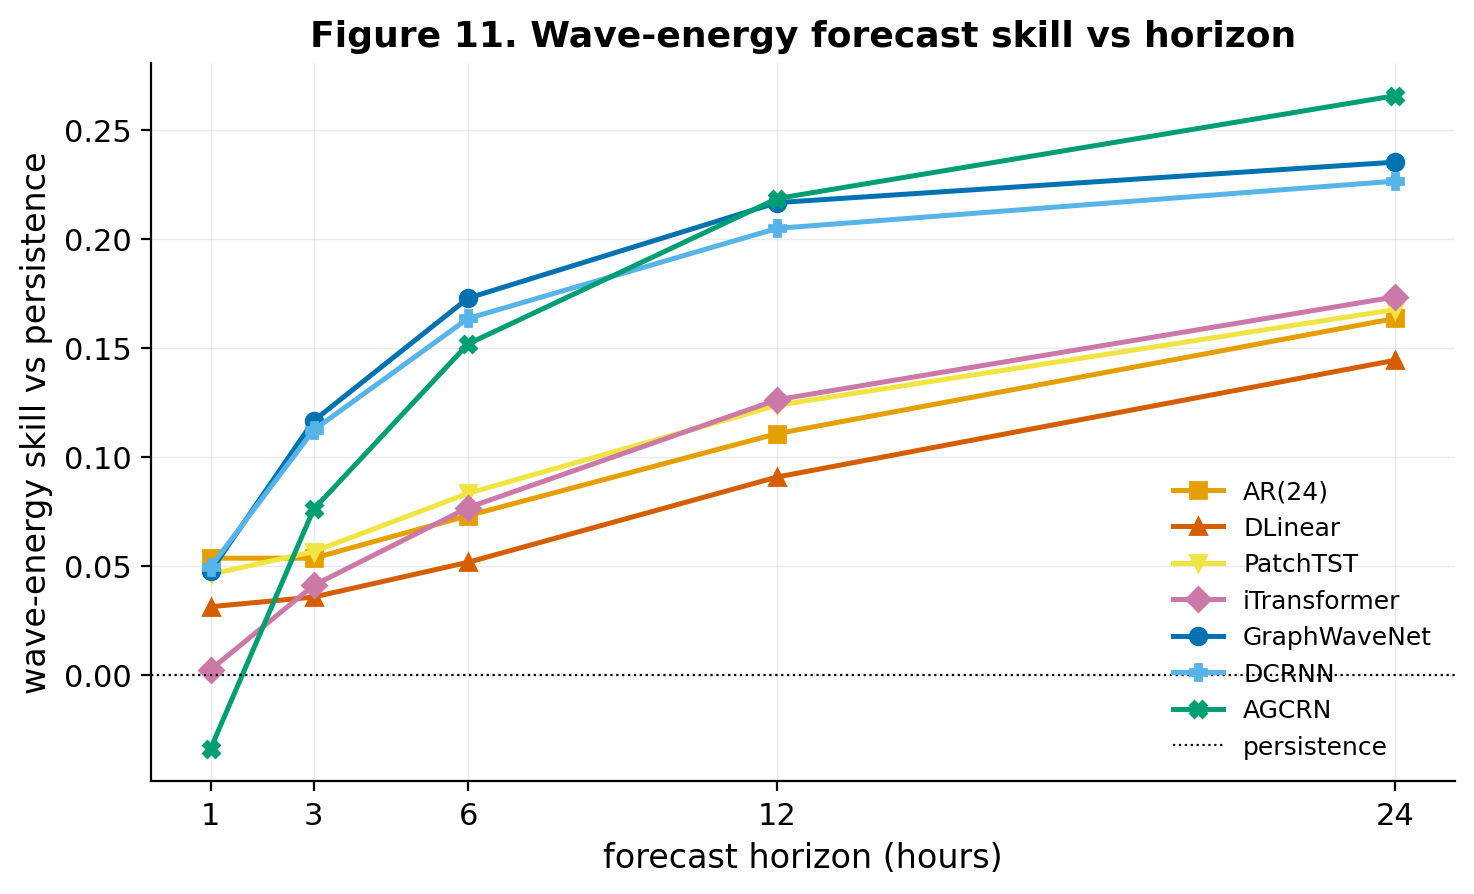
\includegraphics[width=\textwidth,height=0.72\textheight,keepaspectratio]{fig11_energy_forecast.png}\end{center}
\end{frame}

\end{document}
